\documentclass[11pt]{elegantbook}
\definecolor{structurecolor}{RGB}{40,58,129}
\linespread{1.6}
\setlength{\footskip}{20pt}
\setlength{\parindent}{0pt}
\newcommand{\argmax}{\operatornamewithlimits{argmax}}
\newcommand{\argmin}{\operatornamewithlimits{argmin}}
\elegantnewtheorem{proof}{Proof}{}{Proof}
\elegantnewtheorem{claim}{Claim}{prostyle}{Claim}
\DeclareMathOperator{\col}{col}
\title{\textbf{Deep Learning}}
\author{Wenxiao Yang}
\institute{Department of Mathematics, University of Illinois at Urbana-Champaign}
\date{2022}
\setcounter{tocdepth}{2}
\cover{cover.jpg}
\extrainfo{All models are wrong, but some are useful.}

% modify the color in the middle of titlepage
\definecolor{customcolor}{RGB}{32,178,170}
\colorlet{coverlinecolor}{customcolor}
\usepackage{cprotect}

\addbibresource[location=local]{reference.bib} % bib

\begin{document}
\maketitle

\frontmatter
\tableofcontents

\mainmatter



\chapter{Learning Basics}
\section{Parameters and Hyperparameters}
\begin{definition}
    \textbf{Parameters} are values learned by the model given the data.
\end{definition}
e.g. $\beta, W, b, \theta$.
\begin{definition}
    \textbf{Hyperparameters} are values supplied to tune the model and cannot be learned from data.
\end{definition}
e.g. Number of Hidden Layers, Neurons, and Epochs to Train. Learning Rate, and Batch Size.

\section{Neural Network: Back Propagation Algorithm}
\underline{\textbf{Neural Network}}
\begin{center}\begin{figure}[htbp]
    \centering
    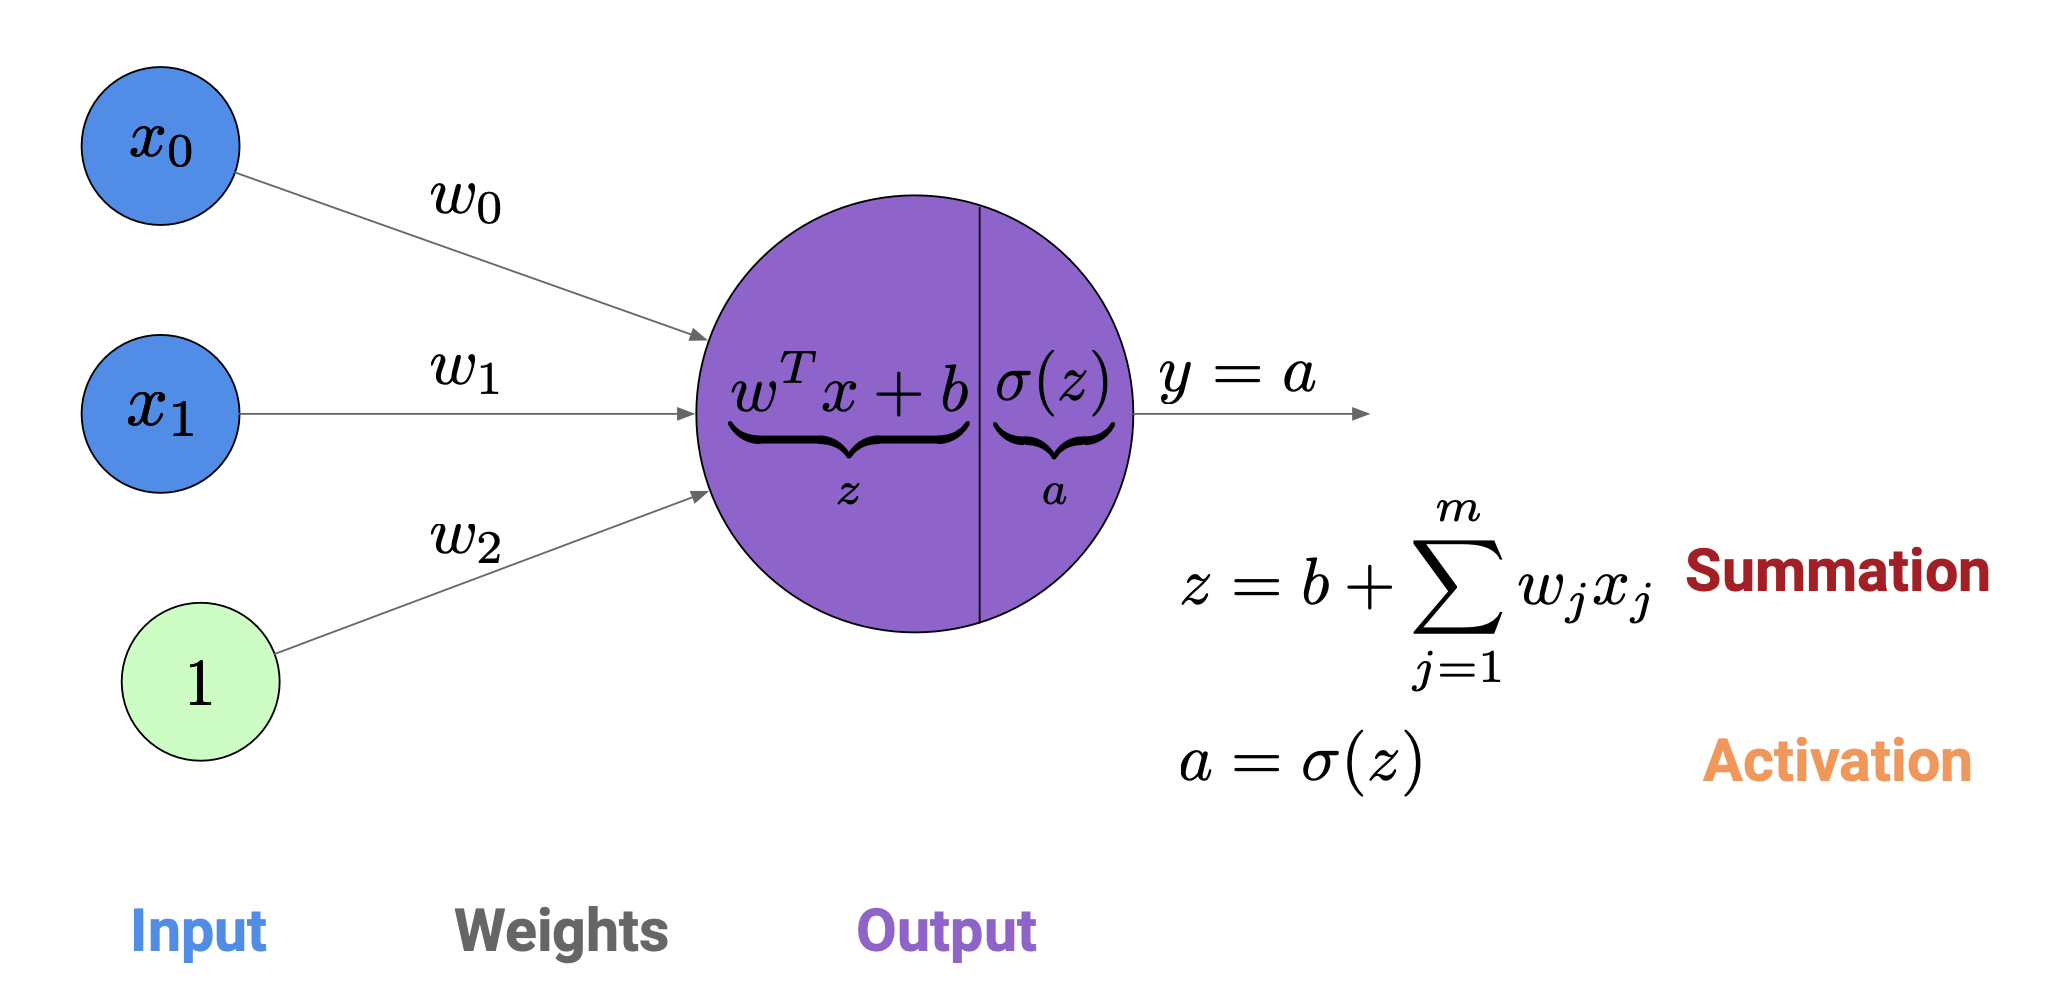
\includegraphics[scale=0.2]{neuron1.png}
    \caption{Simple Neural Network}
    \label{}
\end{figure}\end{center}
Given a vector input $x$, we need to find the best estimator $\hat{y}$ which minimizes lost function. In the figure that has only one layer and one pathway, we find the parameter $(\omega,b)$ to form an input $\omega^Tx+b$ to neuron $\sigma$ (activation function).  Then, the final output (estimator) of the network is $\hat{y}=\sigma(\omega^Tx+b)$.


\subsection{Activations}
\begin{definition}
    \underline{Activation functions} are element-wise gates for letting information propagate to future layers either transformed with non-linearities or left as-is.
\end{definition}
\textbf{Example of activation function:}
\begin{center}\begin{figure}[htbp]
    \centering
    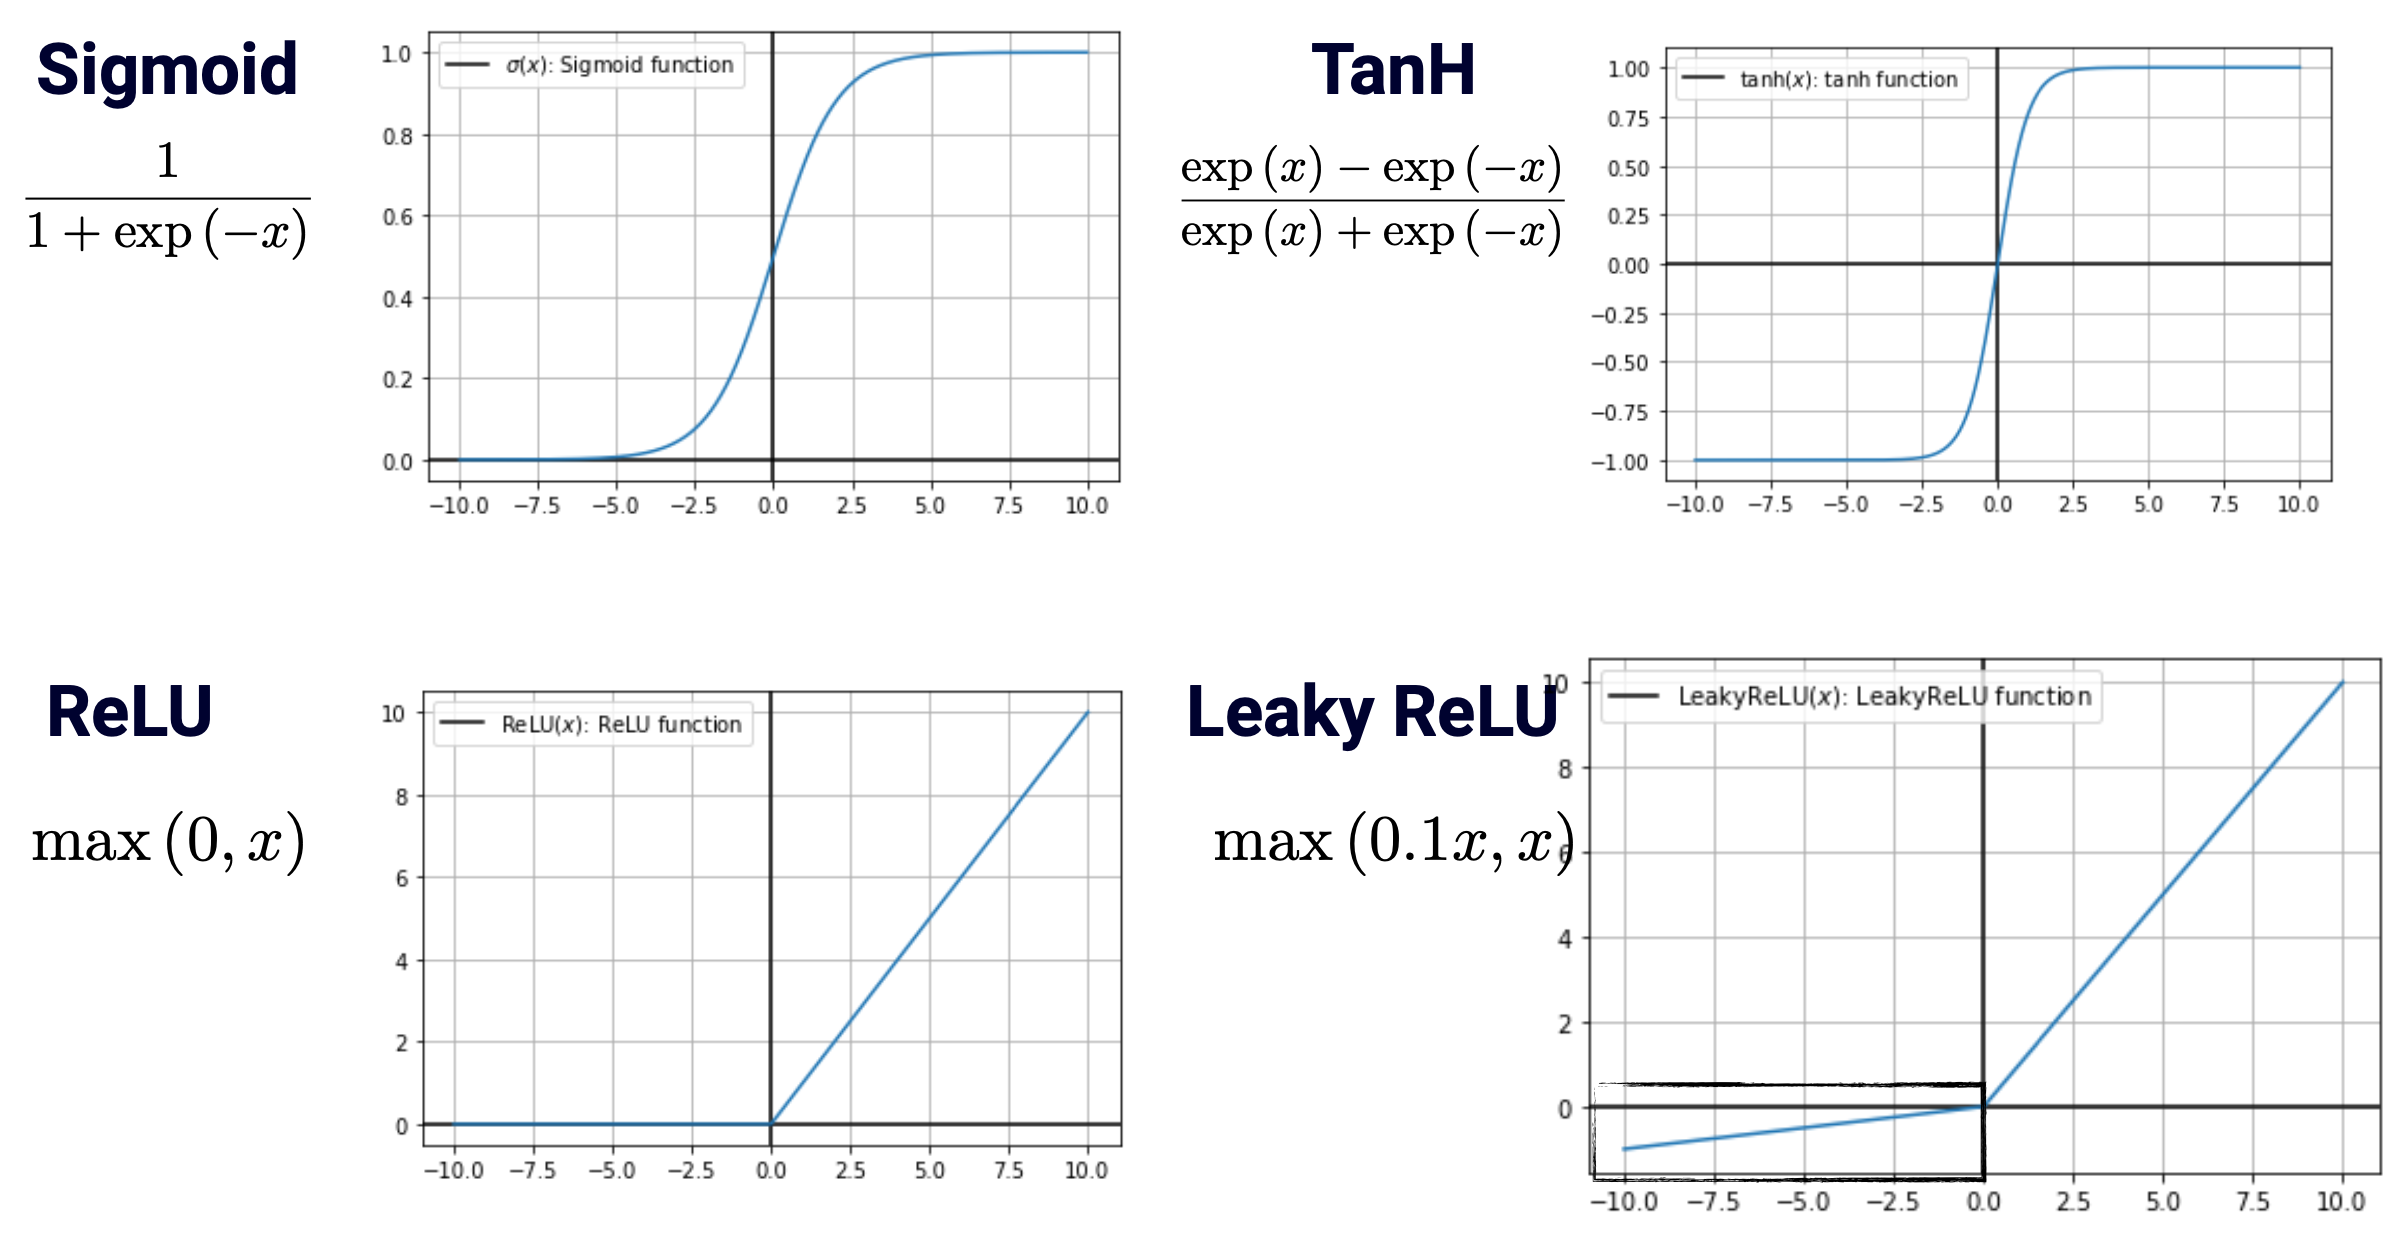
\includegraphics[scale=0.2]{activations.png}
    \caption{Activations}
    \label{}
\end{figure}\end{center}
\begin{enumerate}[(1)]
    \item \textbf{Identity:} $$\text{identity}(x)=I(x)=x$$
    \item \textbf{Binary:} $$\text{binary}(x)=\text{step}(x)=\left\{\begin{matrix}
        1,&x\geq 0\\
        0,&x<0
    \end{matrix}\right.$$
    \item \textbf{Sigmoid:}$$\sigma(x)=\frac{1}{1+e^{-x}}$$
    \begin{equation}
        \begin{aligned}
            \sigma(-x)=1-\sigma(x);\
            \frac{d\sigma(x)}{dx}=\sigma(x)\cdot(1-\sigma(x))
        \end{aligned}
        \nonumber
    \end{equation}
    \begin{equation}
        \begin{aligned}
            \frac{\partial \sigma(\vec{x})}{\partial \vec{x}}=\begin{bmatrix}
                \sigma(x_1)(1-\sigma(x_1)) &\cdots&0\\
                \vdots&\ddots&\vdots\\
                0&\cdots&\sigma(x_n)(1-\sigma(x_n))
            \end{bmatrix}=\text{diag}(\sigma(\vec{x})\cdot (1-\sigma(\vec{x})))
        \end{aligned}
        \nonumber
    \end{equation}
    \item \textbf{TanH:} $$tanh(x)=\frac{e^x-e^{-x}}{e^x+e^{-x}}$$(TanH is a rescaled sigmoid) $$tanh(x)=\frac{e^{2x}-1}{e^{2x}+1}=1-2\sigma(-2x)=2\sigma(2x)-1$$
    \item \textbf{ReLU:} $$g(x)=\max(0,x)$$
    \item \textbf{Leaky ReLU:} $$g(x)=\max(0.1x,x)$$
    \item \textbf{Softmax:} $S_j(\vec{x})=\frac{e^{x_j}}{\sum_{i=1}^ne^{x_i}}$, $$S(\vec{x})=\left[\frac{e^{x_1}}{\sum_{i=1}^ne^{x_i}},\frac{e^{x_2}}{\sum_{i=1}^ne^{x_i}},\cdots, \frac{e^{x_n}}{\sum_{i=1}^ne^{x_i}}\right]^T$$
    $$\frac{\partial S_j(\vec{x})}{\partial x_j}=S_j(\vec{x})[1-S_j(\vec{x})]$$
\end{enumerate}


\subsection{Multilayer Neural Network}
\begin{center}\begin{figure}[htbp]
    \centering
    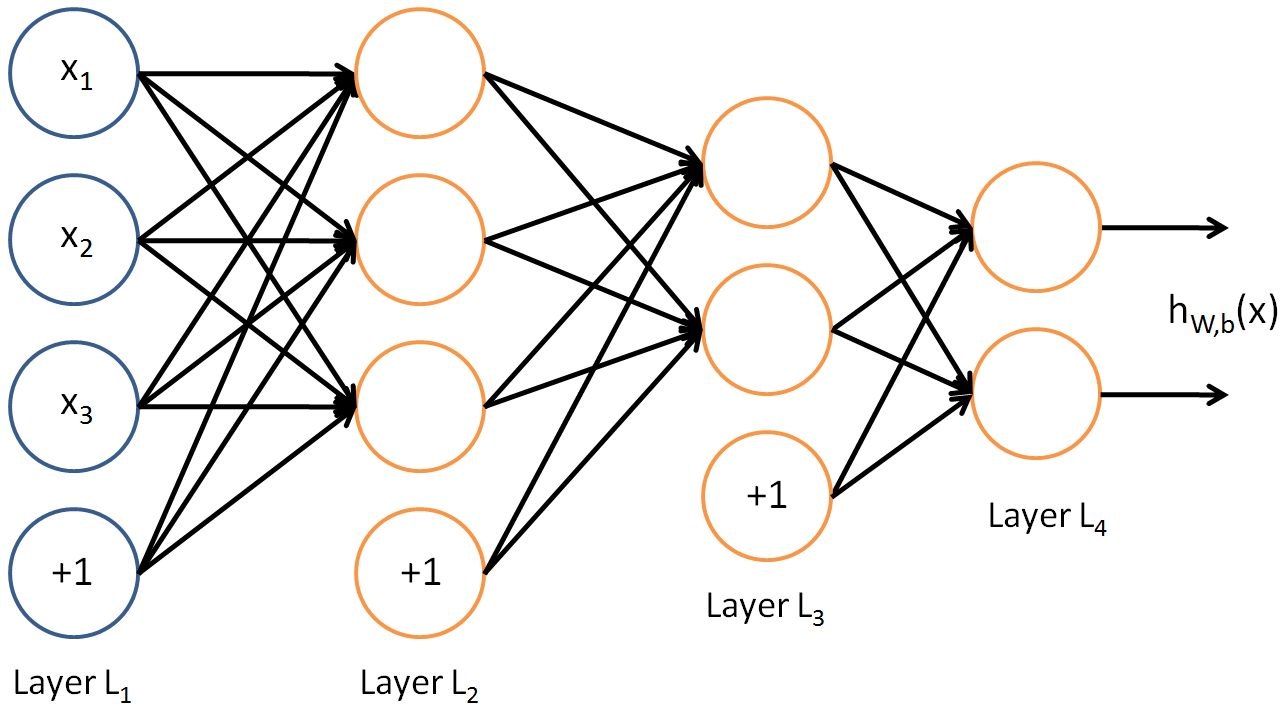
\includegraphics[scale=0.2]{MNN.png}
    \caption{Multilayer Neural Network}
    \label{}
\end{figure}\end{center}
\begin{enumerate}[$\bullet$]
    \item Number of neurons in each layer can be different.
    \item All weights on edge connecting layers $m-1$ and $m$ is matrix $W^{(m)}$, with $w_{ij}^{(m)}$ being the weight connecting output $j$ of layer $m-1$ with neuron $i$ of layer $m$.
    \item Input to network is vector $x$; output of layer $m$ is vector $y^{(m)}$
    \begin{equation}
        \begin{aligned}
            y_i^{(1)}=\sigma(x_i^{(1)}),&\text{ with }x_i^{(1)}=\sum_jw_{ij}^{(1)}x_j+b_i^{(1)}\\
            y^{(1)}=\sigma(x^{(1)}),&\text{ with }x^{(1)}=W^{(1)}x+b^{(1)}\\
            y^{(2)}=\sigma(x^{(2)}),&\text{ with }x^{(2)}=W^{(2)}y^{(1)}+b^{(2)}\\
            \vdots&\\
            y^{(M)}=\sigma(x^{(M)}),&\text{ with }x^{(M)}=W^{(M)}y^{(M-1)}+b^{(M)}\\
        \end{aligned}
        \nonumber
    \end{equation}
\end{enumerate}

We want to find the weights $W^{(1)},\cdots,W^{(M)},b^{(1)},\cdots,b^{(M)}$ so that the output of last layer
\begin{equation}
    \begin{aligned}
        \hat{y}=y^{(M)}\approx f^*(x)=y
    \end{aligned}
    \nonumber
\end{equation}
$f^*(x)$ is the unknown thing we need to predict.

We use \underline{labelled training data}, i.e.
\begin{equation}
    \begin{aligned}
        (x[1],y[1]),(x[2],y[2]),\cdots (x[N],y[N])
    \end{aligned}
    \nonumber
\end{equation}
Minimize the "empirical" loss on training data.
\begin{equation}
    \begin{aligned}
        J=\sum_{i=1}^N L(y[i],\hat{y}[i])
    \end{aligned}
    \nonumber
\end{equation}
where $\bar{y}[i]$ is the output of NN whose input is $x[i]$.

\begin{enumerate}[$\bullet$]
    \item $L$ is the function of $W^{(1)},\cdots,W^{(M)},b^{(1)},\cdots,b^{(M)}$ to measure the loss. e.g. the square loss $$L(y,\hat{y})=(y-\hat{y})^2$$
    \item We wish to minimize $J$ using a \underline{gradient descent procedure}.
    \item To compute gradient we need:
    \begin{equation}
        \begin{aligned}
            \frac{\partial L}{\partial w_{ij}^{(l)}}\text{ for each }l,i,j; \quad
            \frac{\partial L}{\partial b_i^{(l)}}\text{ for each }l,i.\\
        \end{aligned}
        \nonumber
    \end{equation}
\end{enumerate}

\subsection{A Simple Example of Back Propagation Algorithm}
We can consider a simple example (one layer, two pathways)
\begin{center}\begin{figure}[htbp]
    \centering
    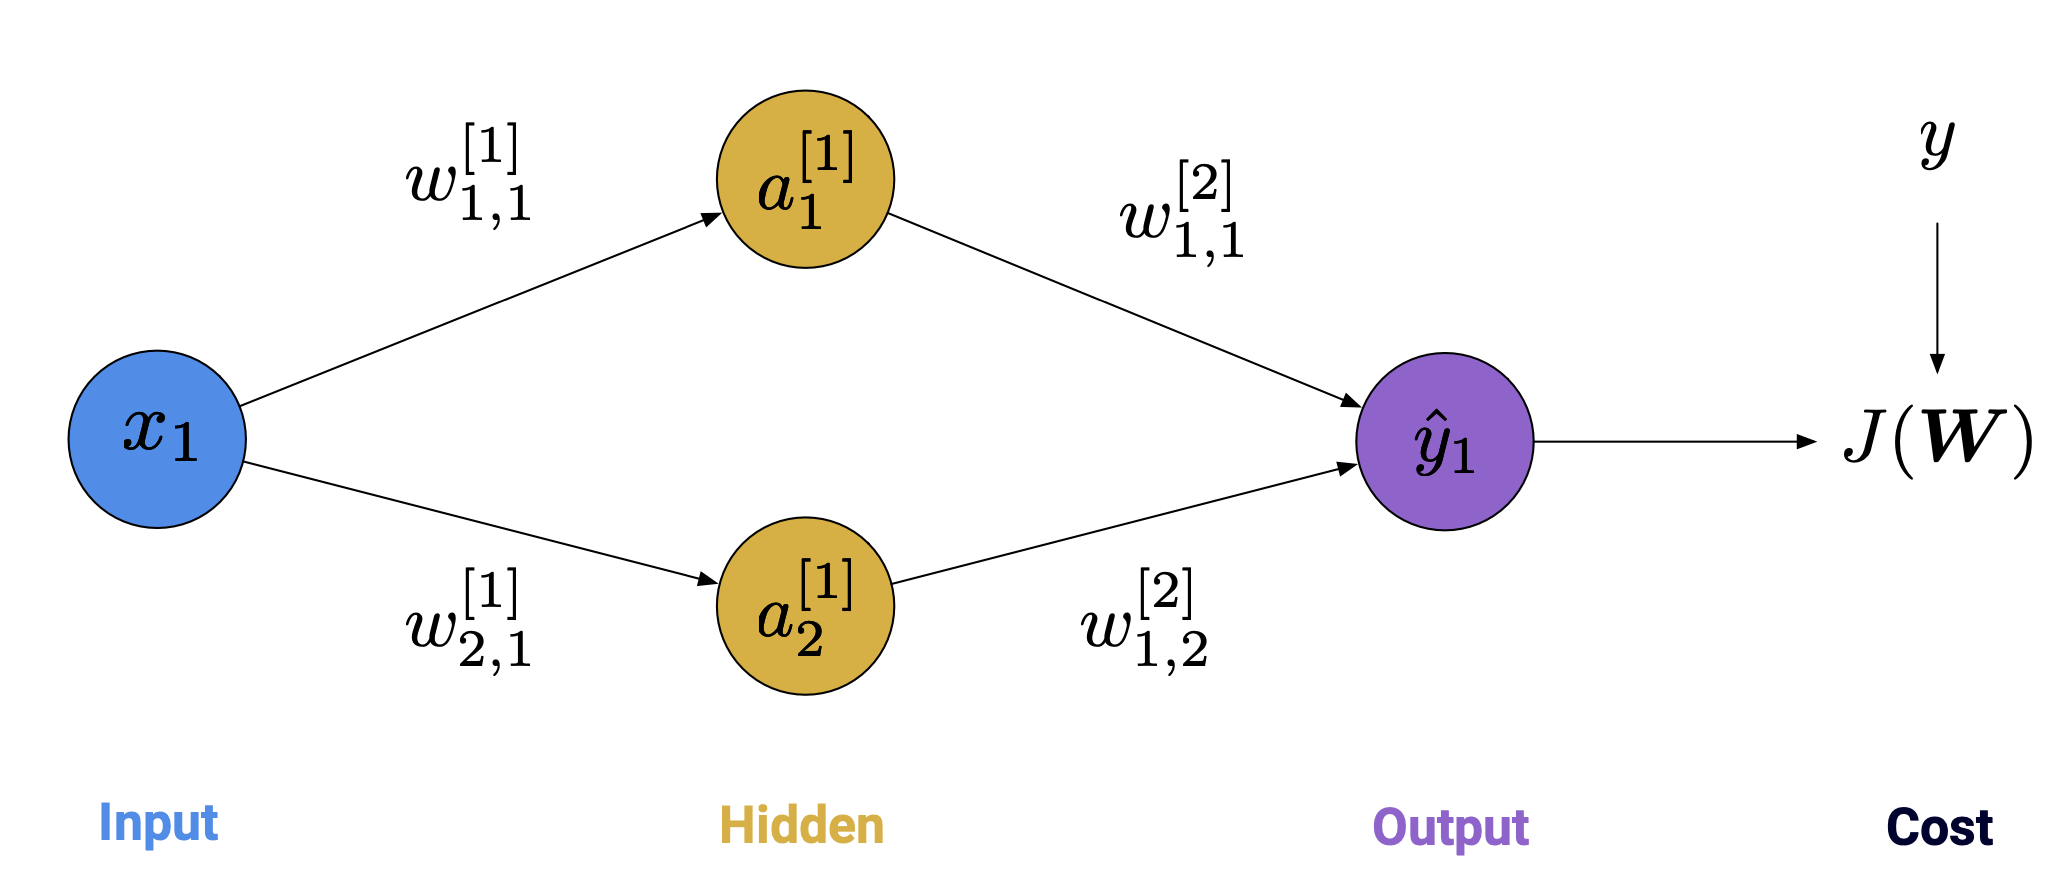
\includegraphics[scale=0.2]{2path.png}
    \caption{Two Independent Pathways}
    \label{}
\end{figure}\end{center}
$W^{(1)}=[w_{1,1}^{[1]},w_{2,1}^{[1]}]^T$, $b^{(1)}=[0,0]^T$, $\sigma_1(x)=x$.

$W^{(2)}=[w_{1,1}^{[2]},w_{1,2}^{[2]}]$, $b^{(2)}=0$, $\sigma_2(x)=x$.

\begin{equation}
    \begin{aligned}
        [a_1^{[1]},a_2^{[1]}]^T&=\sigma_1(W^{(1)}x_1+b^{(1)})=[w_{1,1}^{[1]}x_1,w_{2,1}^{[1]}x_1]^T\\
        \hat{y}&=\sigma_2(W^{(2)}[a_1^{[1]},a_2^{[1]}]^T+b^{(2)})=(w_{1,1}^{[1]}w_{1,1}^{[2]}+w_{2,1}^{[1]}w_{1,2}^{[2]})x_1
    \end{aligned}
    \nonumber
\end{equation}

\begin{equation}
    \begin{aligned}
        \frac{\partial J(\hat{y})}{\partial w_{2,1}^{[1]}}=\frac{\partial J(\hat{y})}{\partial \hat{y}}\cdot \frac{\hat{y}}{\partial a_2^{[1]}}\cdot\frac{a_2^{[1]}}{\partial w_{2,1}^{[1]}}
    \end{aligned}
    \nonumber
\end{equation}

\subsection{Back Propagation Algorithm}
Recall $y_i^{(m)}=\sigma(x_i^{(m)})$, $x_i^{(m)}=\sum_jw_{ij}^{(m)}y_j^{(m-1)}+b_i^{(m)}$
\begin{equation}
    \begin{aligned}
        \frac{\partial L}{\partial w_{ij}^{(m)}}=\frac{\partial L}{\partial y_i^{(m)}}\cdot \frac{\partial y_i^{(m)}}{\partial w_{ij}^{(m)}}=\frac{\partial L}{\partial y_i^{(m)}}\cdot \frac{\partial y_i^{(m)}}{\partial x_{i}^{(m)}}\cdot \frac{\partial x_{i}^{(m)}}{\partial w_{ij}^{(m)}}
    \end{aligned}
    \nonumber
\end{equation}
\begin{equation}
    \begin{aligned}
        \frac{\partial L}{\partial b_{i}^{(m)}}&=\frac{\partial L}{\partial y_i^{(m)}}\cdot \frac{\partial y_i^{(m)}}{\partial x_{i}^{(m)}}\cdot \frac{\partial x_{i}^{(m)}}{\partial b_{i}^{(m)}}\\
    \end{aligned}
    \nonumber
\end{equation}

\textbf{\underline{For large $M$}},
\begin{enumerate}[$\bullet$]
    \item $\frac{\partial L}{\partial y_i^{(M)}}$ is easy to compute.
    \item $\frac{\partial y_i^{(M)}}{\partial x_{i}^{(M)}}=\frac{\partial \sigma(x_{i}^{(M)})}{\partial x_{i}^{(M)}}=\sigma'(x_{i}^{(M)})$, (assuming $\sigma$ differentiable).
    \item $\frac{\partial x_{i}^{(M)}}{\partial w_{ij}^{(M)}}=y_j^{(M-1)}$
\end{enumerate}
Thus,
\begin{equation}
    \begin{aligned}
        \frac{\partial L}{\partial w_{ij}^{(M)}}=\frac{\partial L}{\partial y_i^{(M)}}\cdot \sigma'(x_{i}^{(M)}) \cdot y_j^{(M-1)}
    \end{aligned}
    \nonumber
\end{equation}
Similarly,
\begin{equation}
    \begin{aligned}
        \frac{\partial L}{\partial b_{i}^{(M)}}&=\frac{\partial L}{\partial y_i^{(M)}}\cdot \frac{\partial y_i^{(M)}}{\partial x_{i}^{(M)}}\cdot \frac{\partial x_{i}^{(M)}}{\partial b_{i}^{(M)}}\\
        &=\frac{\partial L}{\partial y_i^{(M)}}\cdot \sigma'(x_{i}^{(M)})
    \end{aligned}
    \nonumber
\end{equation}

\textbf{\underline{For $1\leq m< M$}}, in this situation $\frac{\partial L}{\partial y_i^{(m)}}$ is not easy to compute. Note that $x^{(m+1)}=W^{(m+1)}y^{(m)}+b^{(m+1)}$.
\begin{equation}
    \begin{aligned}
    \frac{\partial L}{\partial y_i^{(m)}}&=\sum_k \frac{\partial L}{\partial x_{k}^{(m+1)}}\cdot \frac{\partial x_{k}^{(m+1)}}{\partial y_i^{(m)}}\\
    &=\sum_k \frac{\partial L}{\partial y_{k}^{(m+1)}}\cdot\frac{\partial y_{k}^{(m+1)}}{\partial x_{k}^{(m+1)}}\cdot \frac{\partial x_{k}^{(m+1)}}{\partial y_i^{(m)}}\\
    &=\sum_k \frac{\partial L}{\partial y_{k}^{(m+1)}}\cdot\sigma'(x_k^{(m+1)})\cdot w_{ki}^{(m+1)}\\
    \end{aligned}
    \nonumber
\end{equation}

Then use this form to compute,

(We can set $\delta^{(m)}=\frac{\partial L}{\partial y_i^{(m)}}\cdot \sigma'(x_{i}^{(m)})$ to avoid duplicate computation.)
\begin{equation}
    \begin{aligned}
        \frac{\partial L}{\partial w_{ij}^{(m)}}&=\frac{\partial L}{\partial y_i^{(m)}}\cdot \frac{\partial y_i^{(m)}}{\partial x_{i}^{(m)}}\cdot \frac{\partial x_{i}^{(m)}}{\partial w_{ij}^{(m)}}\\
        &=\frac{\partial L}{\partial y_i^{(m)}}\cdot \sigma'(x_{i}^{(m)}) \cdot y_j^{(m-1)}\\
        &=\delta^{(m)}\cdot y_j^{(m-1)}
    \end{aligned}
    \nonumber
\end{equation}

Similarly,
\begin{equation}
    \begin{aligned}
        \frac{\partial L}{\partial b_{i}^{(m)}}&=\frac{\partial L}{\partial y_i^{(m)}}\cdot \frac{\partial y_i^{(m)}}{\partial x_{i}^{(m)}}\cdot \frac{\partial x_{i}^{(m)}}{\partial b_{i}^{(m)}}\\
        &=\frac{\partial L}{\partial y_i^{(m)}}\cdot \sigma'(x_{i}^{(m)})\\
        &=\delta^{(m)}
    \end{aligned}
    \nonumber
\end{equation}

\begin{center}
    \fcolorbox{black}{gray!10}{\parbox{.9\linewidth}{
\textbf{Summary}
\begin{enumerate}
    \item Compute $\frac{\partial L}{\partial y_i^{(M)}}$.
    \item Use $$\frac{\partial L}{\partial y_i^{(m)}}=\sum_k \frac{\partial L}{\partial y_{k}^{(m+1)}}\cdot\sigma'(x_k^{(m+1)})\cdot w_{ki}^{(m+1)}$$ compute $\frac{\partial L}{\partial y_i^{(m)}}$ for $m=1,2...,M-1$.
    \item Compute $$\frac{\partial L}{\partial b_{i}^{(m)}}=\frac{\partial L}{\partial y_i^{(m)}}\cdot \sigma'(x_{i}^{(m)})=\delta^{(m)}$$ for $m=1,2...,M$.
    \item Compute $$\frac{\partial L}{\partial w_{ij}^{(m)}}=\frac{\partial L}{\partial y_i^{(m)}}\cdot \sigma'(x_{i}^{(m)}) \cdot y_j^{(m-1)}=\delta^{(m)}\cdot y_j^{(m-1)}$$ for $m=1,2...,M$.
\end{enumerate}
    }}
\end{center}

\subsection{Other Methods}
Stochastic Gradient Descent (SGD)

Subgradient Method

\section{Perceptron Algorithm}
\begin{definition}
    \underline{Binary linear classifiers} distinguish between two categories through a linear function of the inputs.
\end{definition}

\begin{definition}
    \underline{Linearly separable} refers to a line that can be drawn to perfectly split the two classes.
\end{definition}

The Perceptron algorithm is an efficient algorithm for learning a \textbf{linear separator} in $d-$dimensional space, with a mistake bound that depends on the margin of separation of the data.
\subsection{General Idea}
Given the training data $$D=\left\{\left\langle x^{(i)},y^{(i)}\right\rangle,i=1,...,n\right\}\in \left(\mathbb{R}^m\times\{0,1\}\right)^n$$ we want to know the exact value of $y\in\{0,1\}$.
\begin{center}\begin{figure}[htbp]
    \centering
    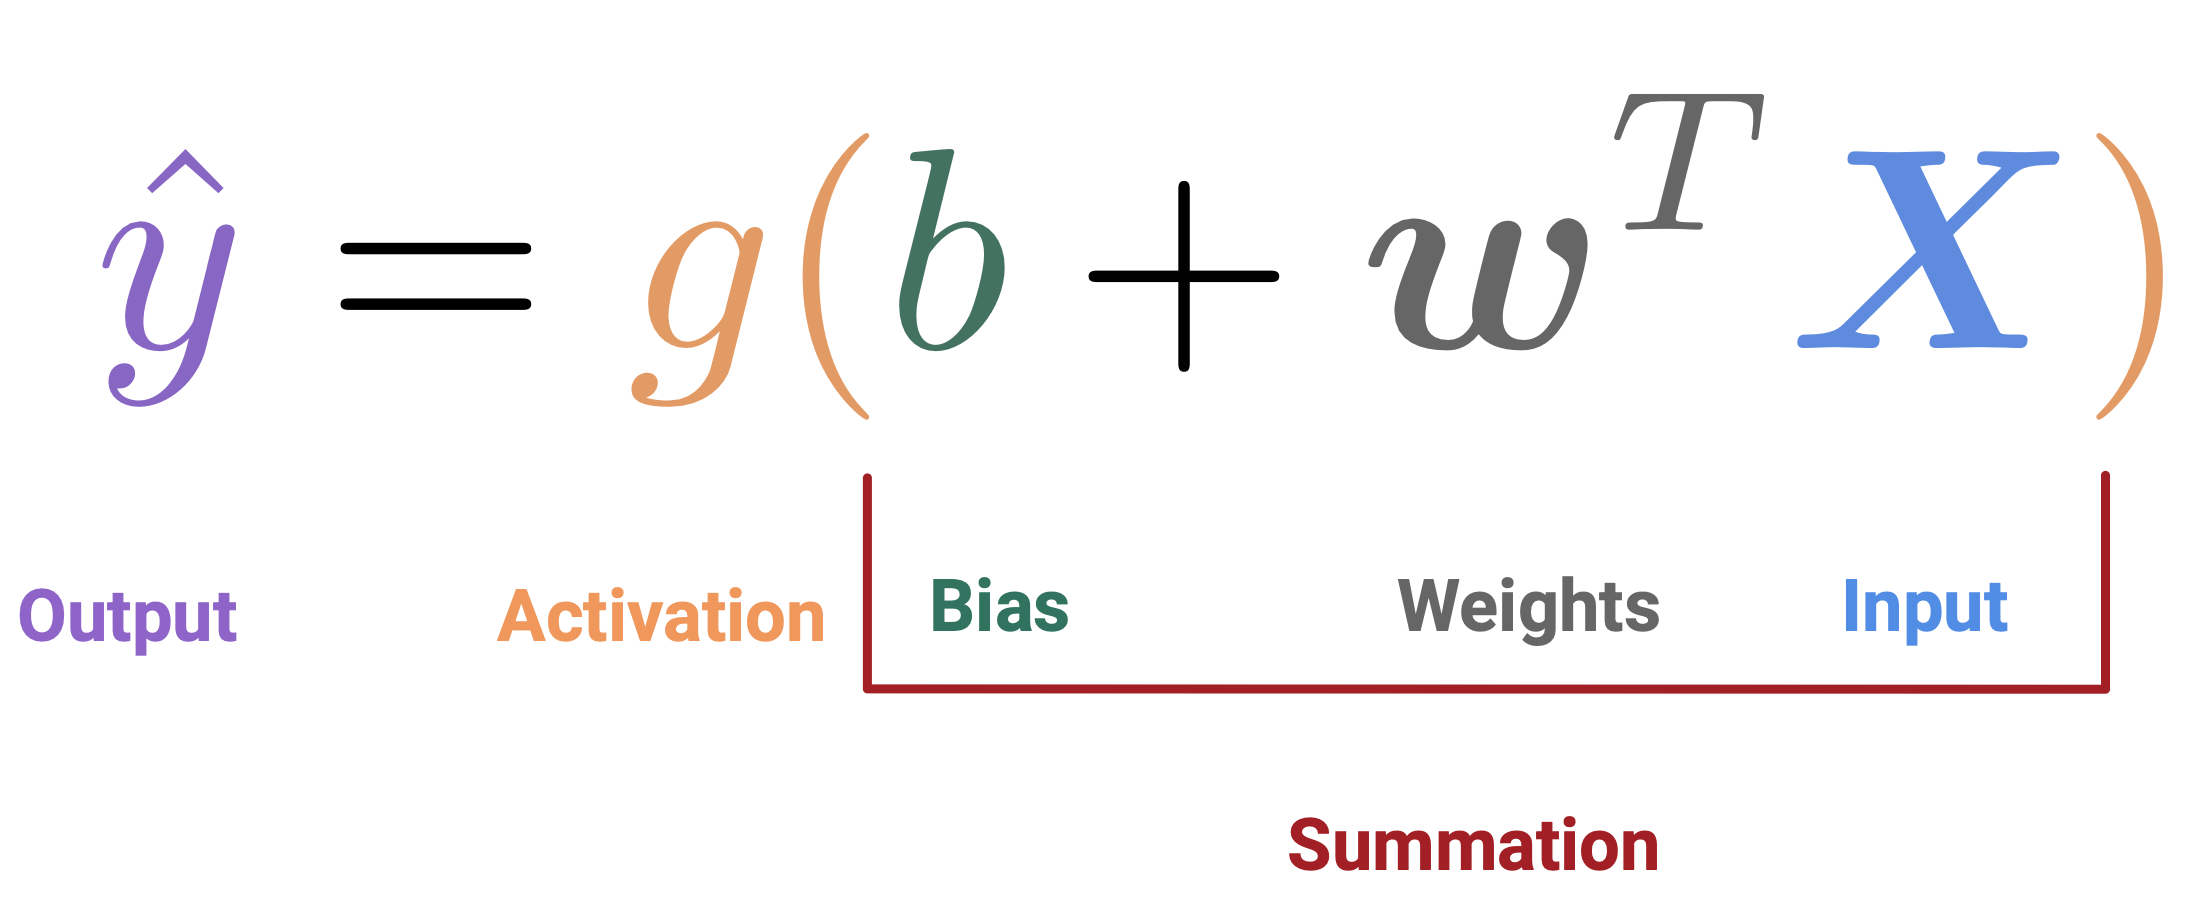
\includegraphics[scale=0.1]{Per_output.png}
    \caption{Perceptron Output}
    \label{}
\end{figure}\end{center}
\begin{center}
    \fcolorbox{black}{gray!10}{\parbox{.9\linewidth}{
    \subsection*{General idea:}
    \begin{enumerate}[$\bullet$]
        \item If the perceptron correctly predicts ($\hat{y}=y$):
        \begin{enumerate}[$\cdot$]
            \item Do nothing
        \end{enumerate}
        \item If the perceptron yields an incorrect prediction ($\hat{y}\neq y$):
        \begin{enumerate}[$\cdot$]
            \item If the prediction is $0$ and truth is $1$ ($\hat{y}=0|y=1 \Rightarrow e=y-\hat{y}=1$), add feature vector to weight vector.
            \item If the prediction is $1$ and truth is $0$ ($\hat{y}=1|y=0 \Rightarrow e=y-\hat{y}=-1$), subtract feature vector from the weight vector.
        \end{enumerate}
    \end{enumerate}
    }}
\end{center}

\begin{center}\begin{figure}[htbp]
    \centering
    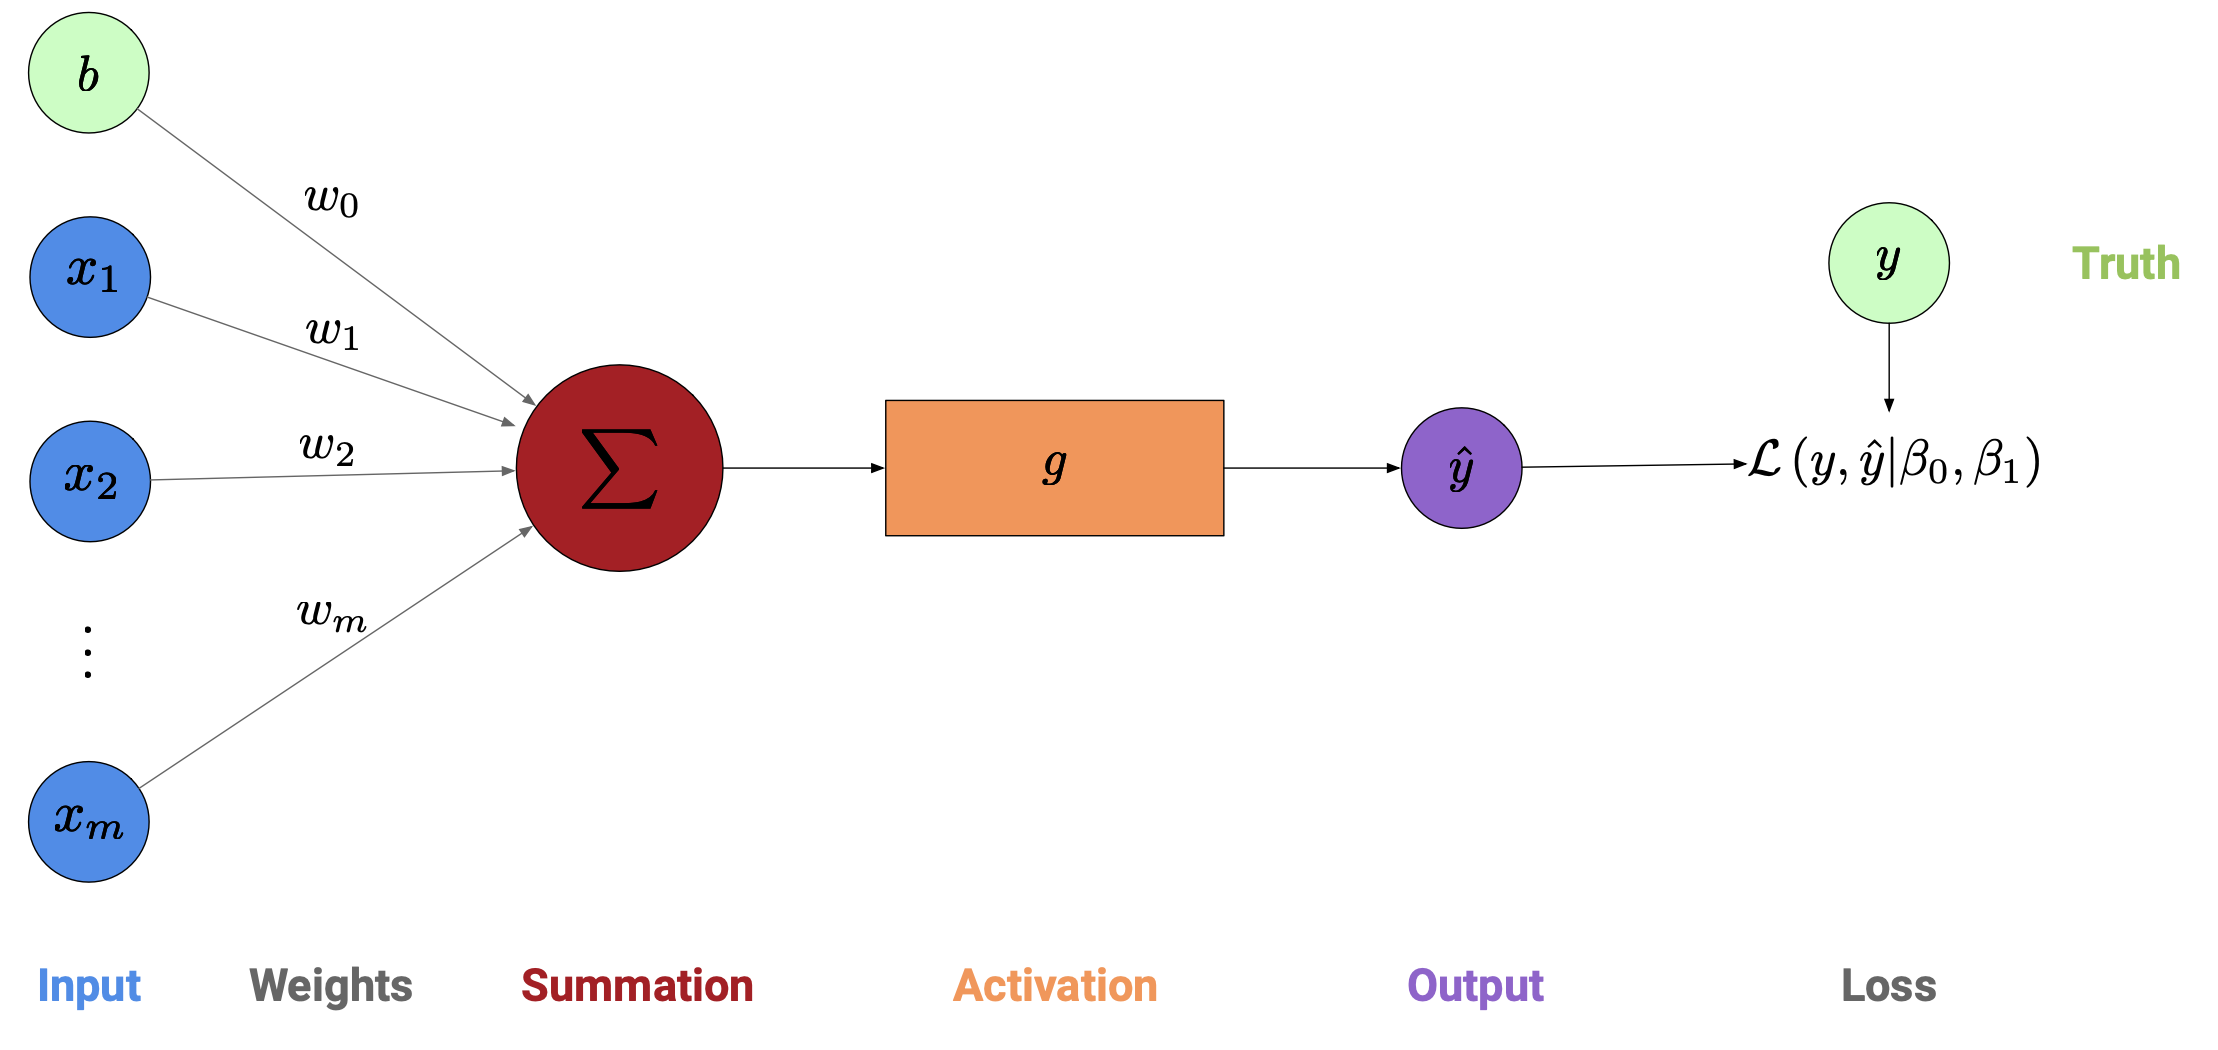
\includegraphics[scale=0.2]{per.png}
    \caption{Perceptron}
    \label{}
\end{figure}\end{center}

Since we want the prediction to be either $0$ or $1$, we usually use binary function as the activation function in perceptron.


\subsection{Algorithm}
\textbf{Perceptron Algorithm:}
\begin{enumerate}[$\bullet$]
    \item Initialize weights (including a bias term) to zero, e.g. $W=[w,b]=0^{m+1}$.
    \item Under each training epoch: Compute for each sample $\left\langle x^{(i)},y^{(i)}\right\rangle\in D$
    \begin{enumerate}[$\cdot$]
        \item A prediction $\hat{y}^{(i)}=g({x^{(i)}}^TW)$
        \item Prediction error $e^{(i)}=y^{(i)}-\hat{y}^{(i)}$
        \item Weighted update $W=W+\eta e^{(i)}x^{(i)}$
    \end{enumerate}
\end{enumerate}

\subsection{Limitations}
\begin{enumerate}[$(1)$]
    \item Only provides a linear classifier boundary.
    \item Only allows for \textbf{binary classifier} between two classes.
    \item \textbf{No convergence possible} if classes are not linearly
    separable.
    \item Perceptron will yield \textbf{multiple boundary/"optimal"
    solutions}.
    \item Boundaries found may \textbf{not} perform \textbf{equally well}.
\end{enumerate}

\section{ADAptive LInear NEuron
(ADALINE)}
\subsection{General Idea}
Except the activation function in perceptron, we can add a threshold function.

In perceptron, we generate the estimation $\hat{y}$ (after binary function) to help update weight $\{w_i\}_{i=0}^m$. However, in ADALINE, we minimize MSE $z=x^TW$ to update weight $\{w_i\}_{i=0}^m$ before output estimation $\hat{y}$ (before binary function).

Before entering threshold (binary function), we want to minimize a mean-
squared error (MSE) loss
function to estimate weights.

e.g. suppose $g(x)=x$, let $z=x^TW$ be the input of threshold, for each $y$,$$W^*=\argmin_{W}L(z,y)=(y-z)^2$$
\begin{equation}
    \begin{aligned}
        \frac{\partial L(z,y)}{\partial w_i}=-2(y-z)\frac{\partial z}{\partial w_i}=-2(y-z)x_i
    \end{aligned}
    \nonumber
\end{equation}

\begin{center}\begin{figure}[htbp]
    \centering
    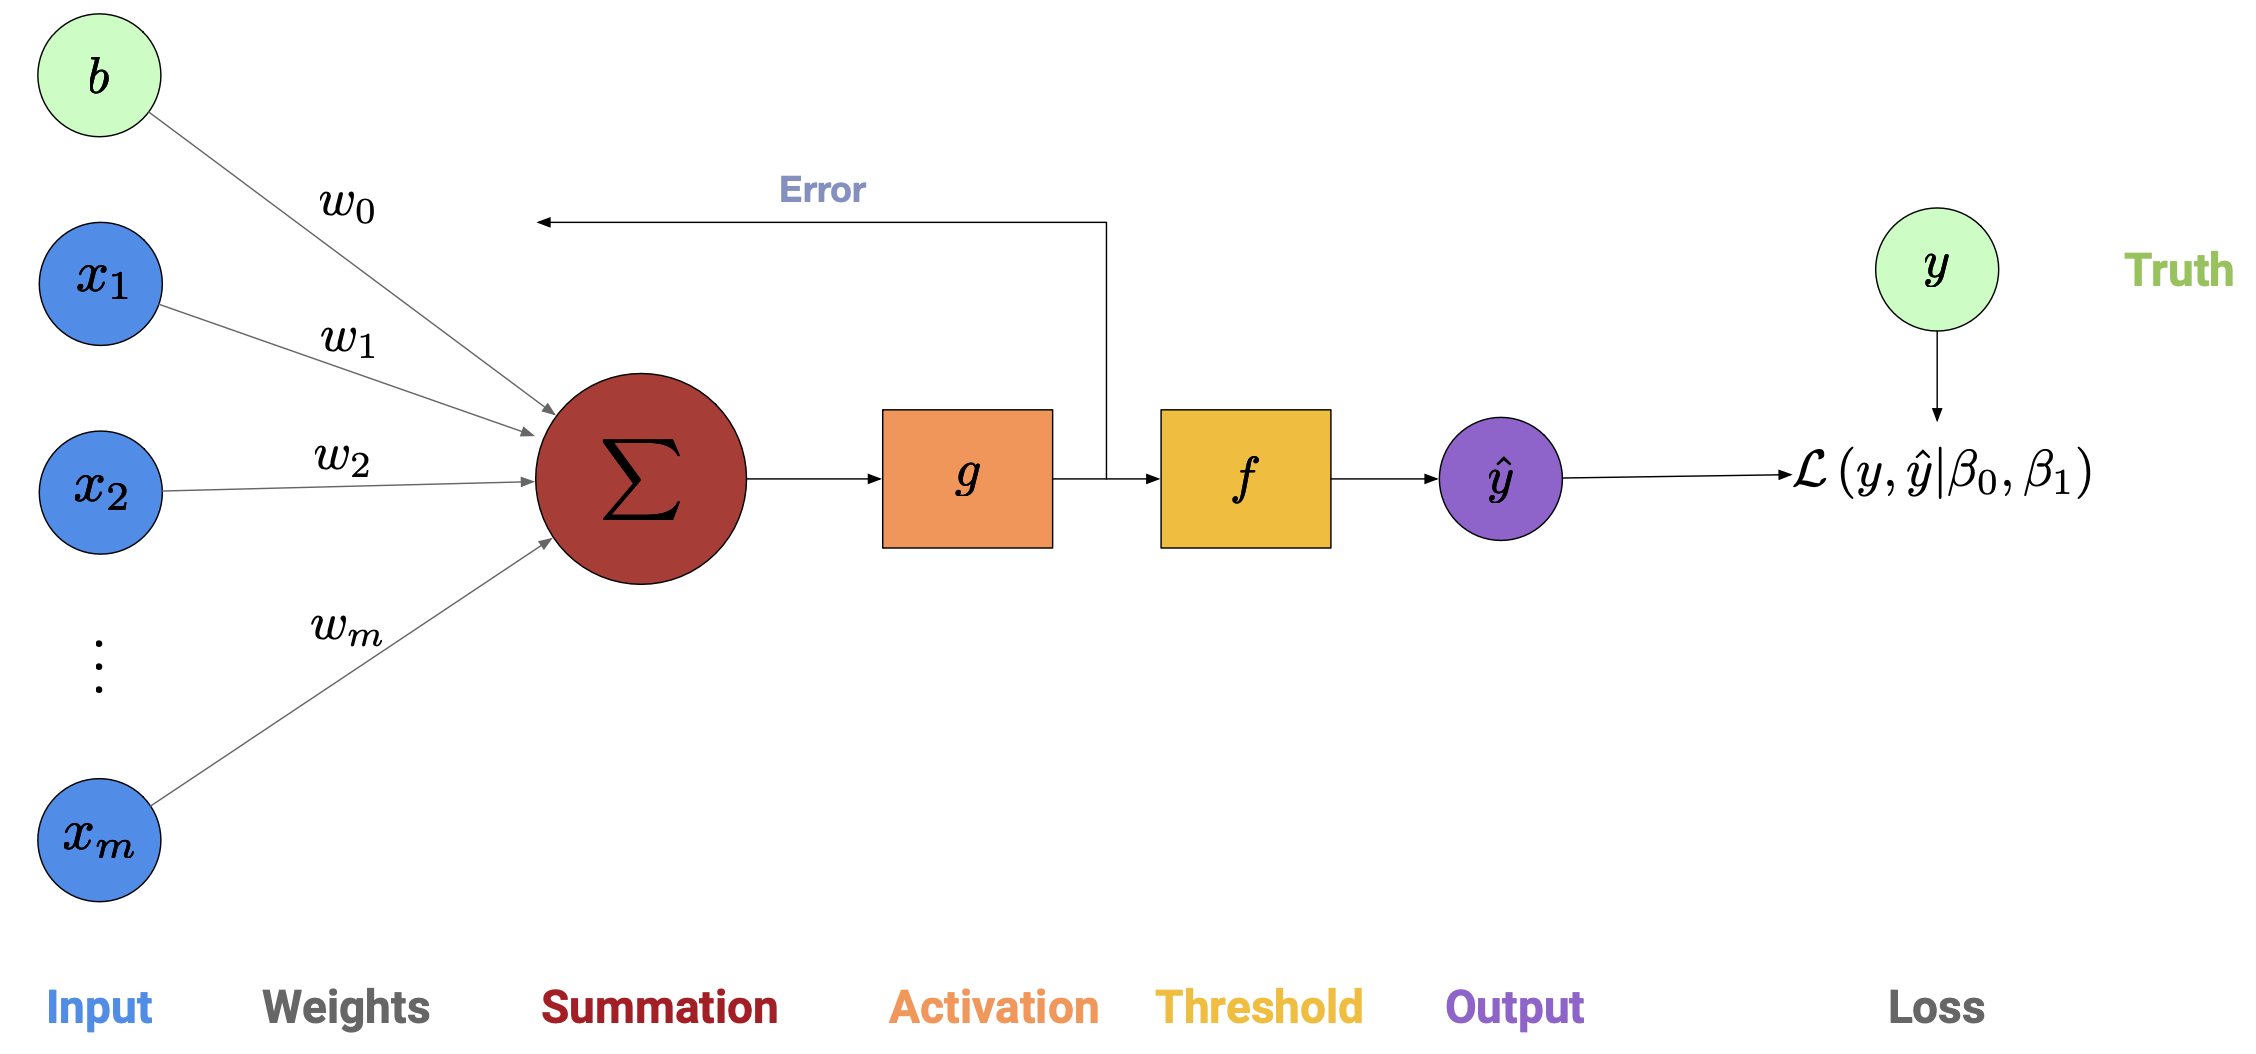
\includegraphics[scale=0.2]{adaline.png}
    \caption{ADALINE}
    \label{}
\end{figure}\end{center}

\subsection{Widrow-Hoff Delta Rule}
(Gradient Descent Rule for ADALINE)
\begin{enumerate}[$\bullet$]
    \item \textbf{Original: }$$W=W+\eta(y^{(j)}-z)x^{(j)}$$
    \item \textbf{Unit-norm: }$$W=W+\eta(y^{(j)}-z)\frac{x^{(j)}}{\|x^{(j)}\|}$$
    where $\|x\|=\sqrt{x_1^2+x_2^2+\cdots+x_m^2}$
\end{enumerate}

\textbf{The Perceptron and ADALINE use variants of the delta rule!}
\begin{enumerate}[(1)]
    \item \textbf{Perceptron}: Output used in delta rule is $\hat{y}=g(x^TW)$; $W=W+\eta(y^{(j)}-{\hat{y}}^{(j)})x^{(j)}$
    \item \textbf{ADALINE}: Output used to estimate weights is $z=x^TW$. $W=W+\eta(y^{(j)}-z)x^{(j)}$
\end{enumerate}

\section{Logistic Regression (Binary-class Output)}
\subsection{Generative and Discriminative Classifiers}
The most important difference between naive Bayes and logistic regression is that \underline{logistic regression} is a \textbf{discriminative classifier} while \underline{naive Bayes} is a \textbf{generative classifier}.

Suppose we want to classify class $A$ (dogs) and class $B$ (cats) (More genearl form: assign a class $c\in C$ to a document $d\in D$):
\begin{enumerate}[(1)]
    \item \underline{\textbf{Generative model:}} A generative model would have the goal of understanding what dogs look like and what cats look like. You might literally ask such a model to ‘generate’, i.e., draw, a dog.\\
    e.g. \textbf{naive Bayes:} we do not directly compute the probability that the document $d$ belongs to each class $c$, $P(c|d)$. We compute likelihood $P(d|c)$ and prior probability $P(c)$ to generate best estimation $\hat{c}$. (i.e., we want to know what should the distribution of a document $d$ in class $c$ be like.) $$\hat{c}=\argmax_{c\in C}P(d|c)P(c)$$
    \item \underline{\textbf{Discriminative model:}} A discriminative model, by contrast, is only trying to learn to distinguish the classes (perhaps without learning much about them). That is we want to directly computing $P(c|d)$.
\end{enumerate}

\subsection{Sigmoid function}
The goal of binary logistic regression is to train a classifier that can make a binary decision about the class of a new input observation.

The input observation is $x=[x_1,...,x_m]^T$ and the output $y$ is either $1$ or $0$. Instead of using the optimal weights of each feature $x_i$ and binary activation function (\textbf{threshold}: $\hat{y}=1$ if $z\geq 0$ and $\hat{y}=0$ otherwise) to estimate  in Perceptron and ADALINE, \textbf{we want to estimate the probability $P(y=1|x)$.}

However, \underline{the weighted sum $z=x^TW=\sum_{i=1}^mw_ix_i+b$ ranges $-\infty$ to $\infty$}. We want to \textbf{force the $z$ to be a legal probability}, that is, to lie between $0$ and $1$.

The \textbf{sigmoid function} $\sigma(z)=\frac{1}{1+e^{-z}}$ can be used as acitivation for this purpose, $P(y=1|x)=\sigma(x^TW)$. Since $1-\sigma(x)=\sigma(-x)$, $P(y=0|x)=\sigma(-x^TW)$.

\subsection{Cross-entropy Loss Function}
We choose the parameters $W$ that maximize the log probability of the true $y$ labels in the training data given the observations $x$. The conditional probability
\begin{equation}
    \begin{aligned}
        p(y|x)=\left\{\begin{matrix}
            \hat{y},&y=1\\
            1-\hat{y},&y=0
        \end{matrix}\right.=\hat{y}^y(1-\hat{y})^{1-y}
    \end{aligned}
    \nonumber
\end{equation}
To maximize the probability, we log both sides:
\begin{equation}
    \begin{aligned}
        \log p(y|x)=y\log\hat{y}+(1-y)\log(1-\hat{y})
    \end{aligned}
    \nonumber
\end{equation}
Then, we want the $\hat{y}$ to maximize the probability (also the logarithm of the probability):
\begin{equation}
    \begin{aligned}
        \hat{y}^*&=\argmax_{\hat{y}\in[0,1]}\log p(y|x)\\
        &=\argmin_{\hat{y}\in[0,1]}-\log p(y|x)\\
        &=\argmin_{\hat{y}\in[0,1]}-(y\log\hat{y}+(1-y)\log(1-\hat{y}))
    \end{aligned}
    \nonumber
\end{equation}
The right hand side is exactly the \textbf{cross-entropy loss function}:
$$L(y,\hat{y})=-(y\log\hat{y}+(1-y)\log(1-\hat{y}))$$
where $\hat{y}^{(i)}=\sigma(w^Tx^{(i)}+b)$
\begin{equation}
    \begin{aligned}
        \frac{\partial L(y^{(i)},\hat{y}^{(i)})}{\partial w_j}=\left(\sigma(w^Tx^{(i)}+b)-y^{(i)}\right)x_j^{(i)}=(\hat{y}^{(i)}-y^{(i)})x_j^{(i)}
    \end{aligned}
    \nonumber
\end{equation}

The risk (Binary Cross-Entropy Cost) of a weight $W$ is $$J(W)=-\frac{1}{n}\sum_{i=1}^n(y^{(i)}\log\hat{y}^{(i)}+(1-y^{(i)})\log(1-\hat{y}^{(i)}))$$
\begin{equation}
    \begin{aligned}
        \frac{\partial J(w,b)}{\partial w_j}=\frac{1}{n}\sum_{i=1}^n\left(\sigma(w^Tx^{(i)}+b)-y^{(i)}\right)x_j^{(i)}
    \end{aligned}
    \nonumber
\end{equation}

\subsection{Algorithm}
\begin{enumerate}[$\bullet$]
    \item Initialize weights (including a bias term) to zero, e.g. $W=[w,b]=0^{m+1}$.
    \item Under each training epoch: Compute for each sample $\left\langle x^{(i)},y^{(i)}\right\rangle\in D$
    \begin{enumerate}[$\cdot$]
        \item A prediction $\hat{y}^{(i)}=g({x^{(i)}}^TW)$
        \item Prediction error $e^{(i)}=y^{(i)}-\hat{y}^{(i)}$
        \item Weighted update $W=W+\eta e^{(i)}x^{(i)}=W-\eta \nabla L(W)$
    \end{enumerate}
\end{enumerate}

\section{Softmax Regression (Multi-class Output)}
\subsection{Multi-Class Classification and Multi-Label Classification}
\begin{definition}
    \underline{Multi-Class Classification} is a process for assigning each sample exactly one class. In this case, classes are considered mutually exclusive (no intersection).
\end{definition}
\begin{center}\begin{figure}[htbp]
    \centering
    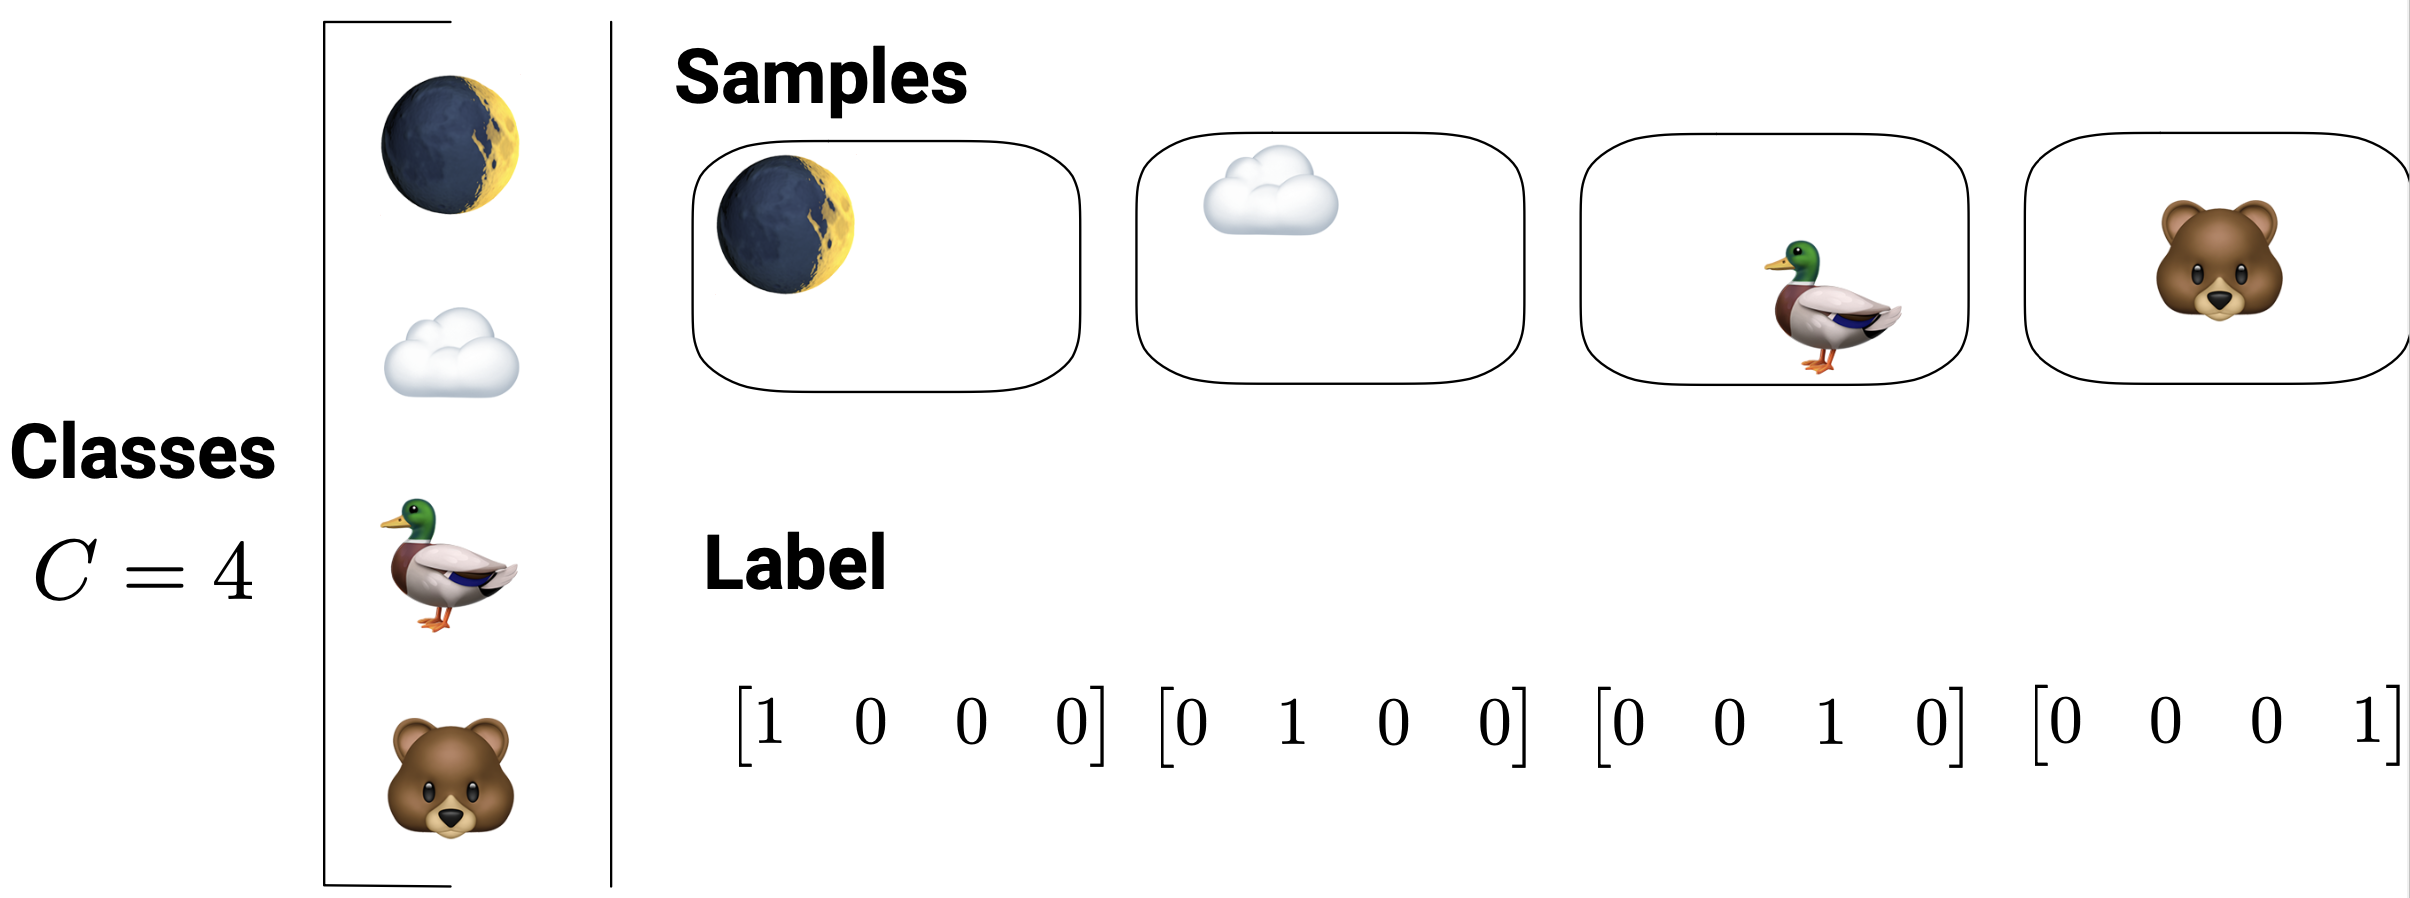
\includegraphics[scale=0.13]{multi-class.png}
    \caption{Multi-Class Classification}
    \label{}
\end{figure}\end{center}
\begin{definition}
    \underline{Multi-Label Classification} or annotation allows for each sample to have 1 or more classes assigned to it. In this case, classes are mutually non-exclusive (one common element).
\end{definition}
\begin{center}\begin{figure}[htbp]
    \centering
    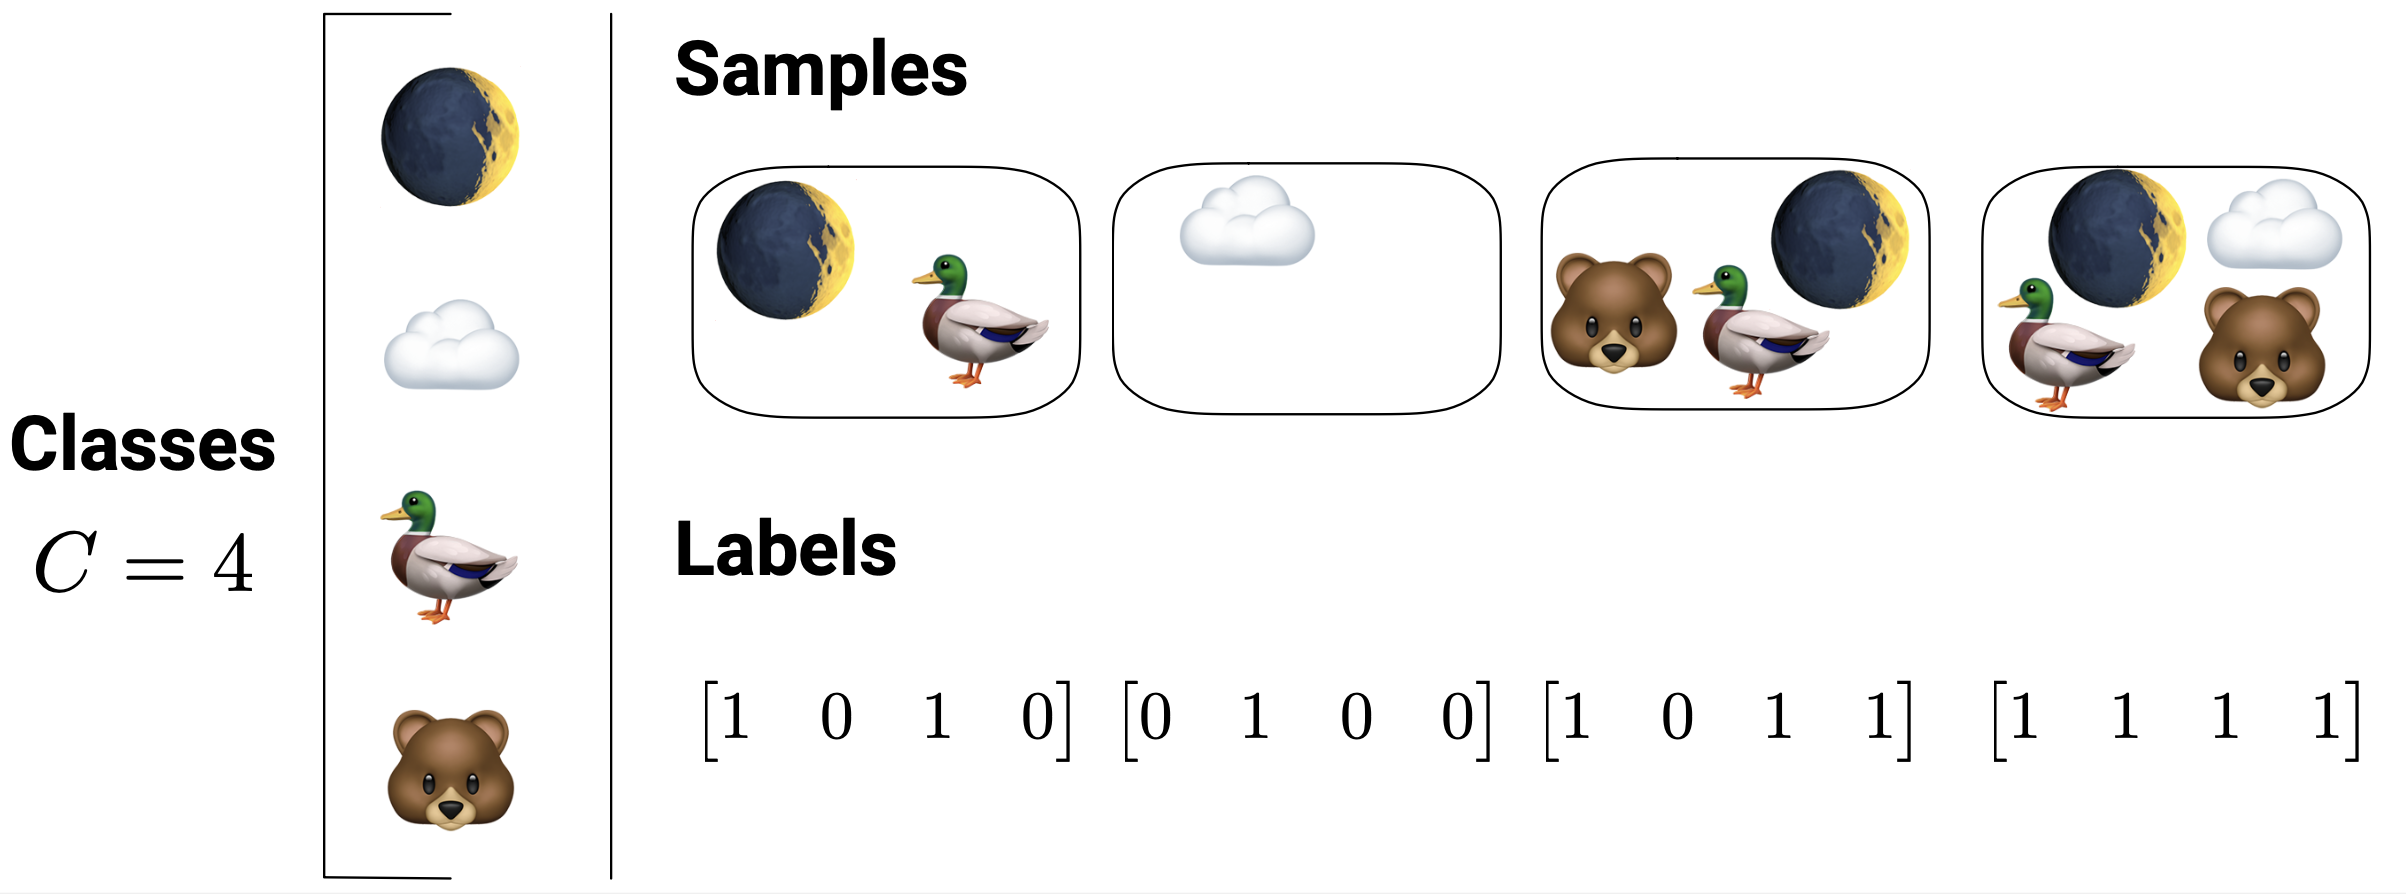
\includegraphics[scale=0.13]{multi-label.png}
    \caption{Multi-Label Classification}
    \label{}
\end{figure}\end{center}

We can show some examples of activation layer and loss choice in different probelms.
\begin{center}\begin{figure}[htbp]
    \centering
    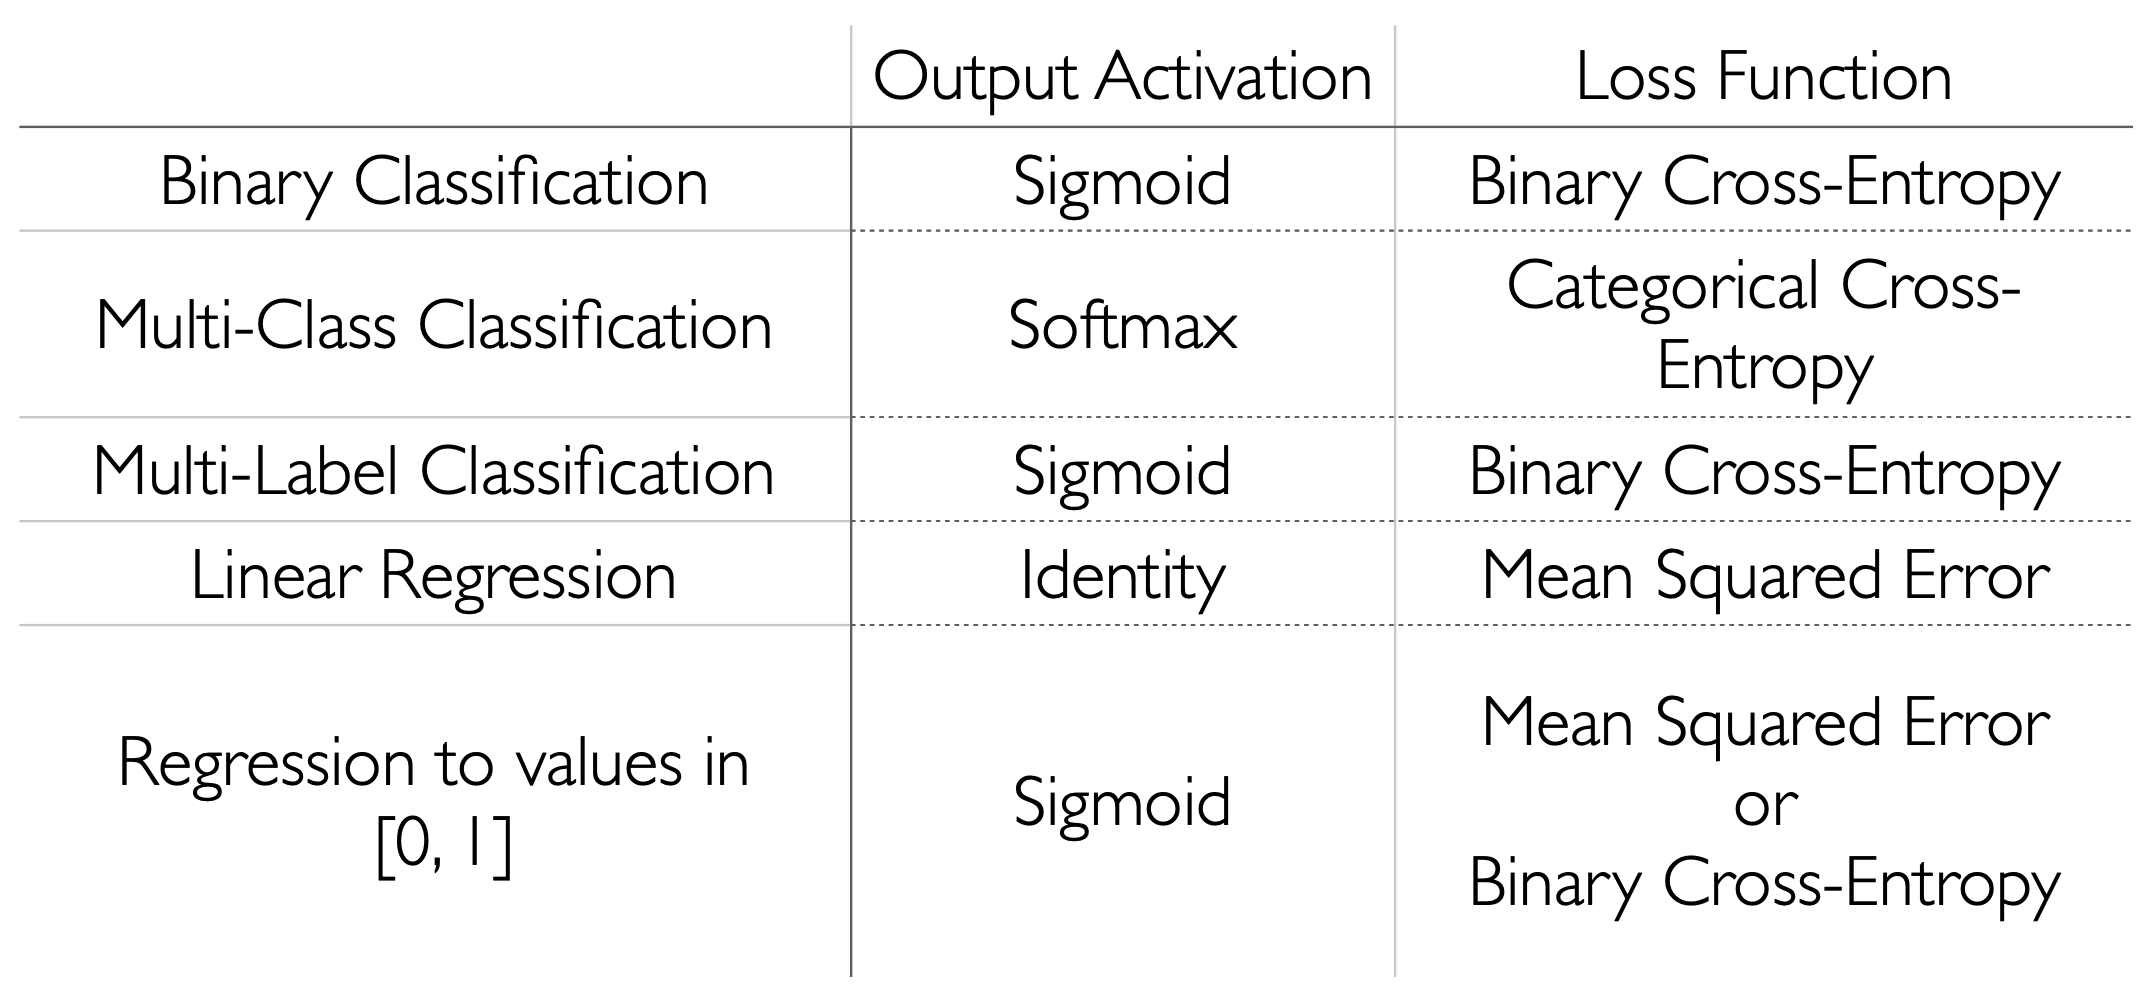
\includegraphics[scale=0.15]{exampleofact.png}
    \caption{Examples of Activation Layer and Loss Choice}
    \label{}
\end{figure}\end{center}

\subsection{One-hot Encoding}
\begin{definition}
    \underline{One-hot encoding} is the process of assigning a single location within a vector to represent a given category.
\end{definition}
\begin{center}\begin{figure}[htbp]
    \centering
    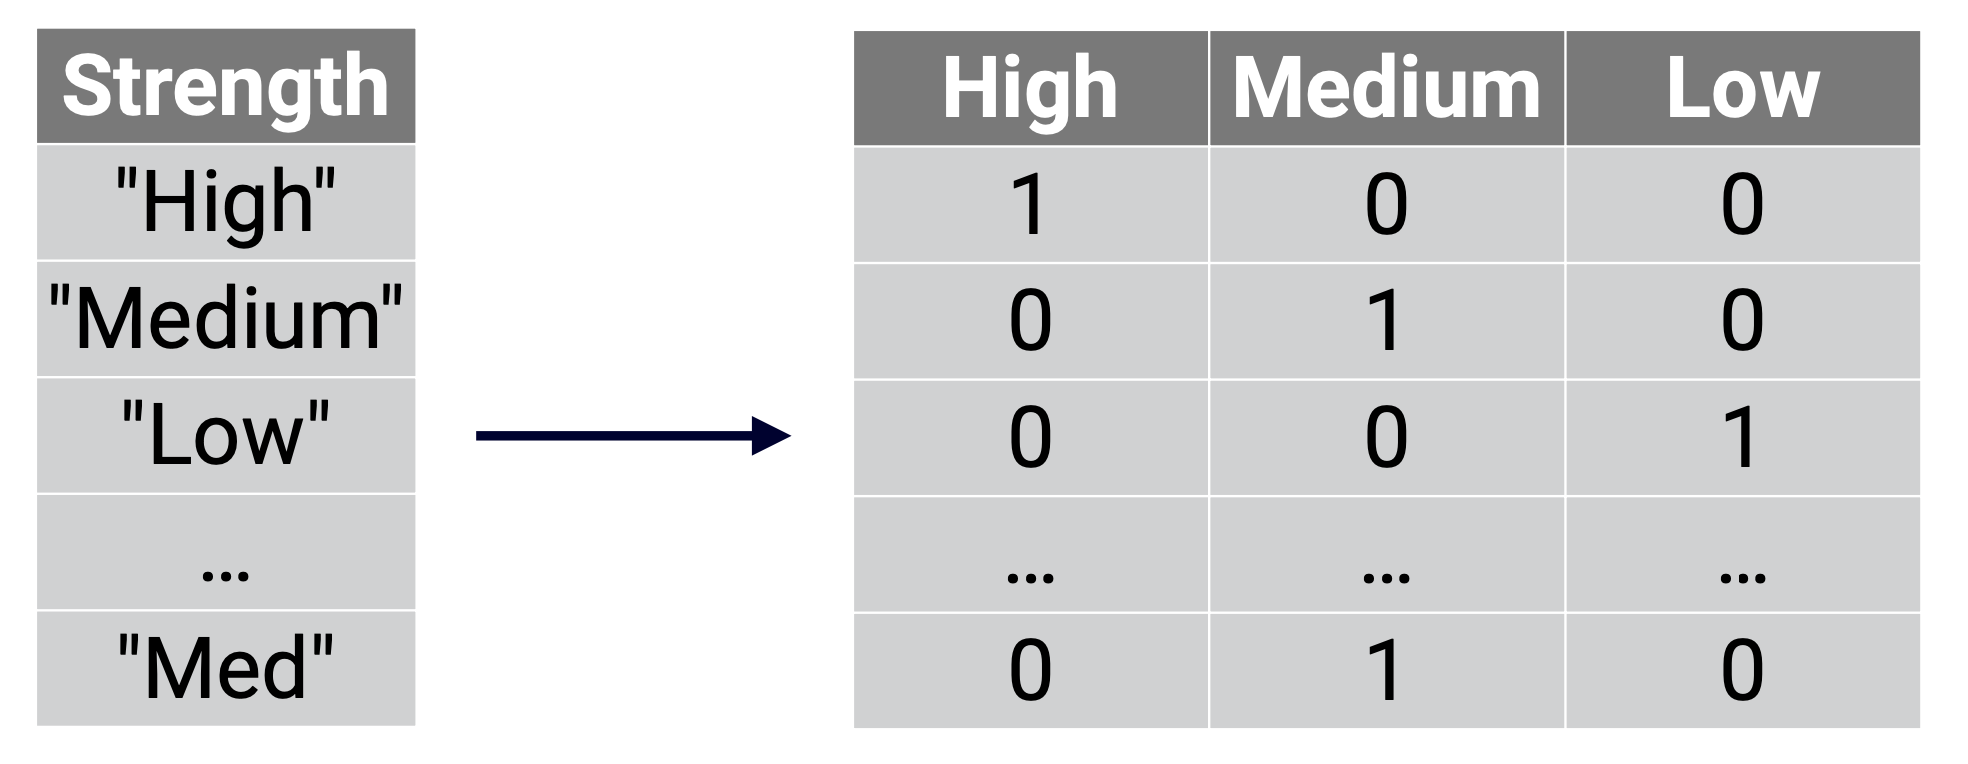
\includegraphics[scale=0.15]{ohe.png}
    \caption{One-hot encoding}
    \label{}
\end{figure}\end{center}
\textbf{Examples:}
\begin{enumerate}
    \item $\mathbf{z}=[4]_{1 \times 1} \rightarrow\left[\begin{array}{lllll}
        0 & 0 & 0 & 0 & 1
        \end{array}\right]_{1 \times 5}$
    \item $\mathbf{y}=\left[\begin{array}{lll}
        3 & 0 & 2
        \end{array}\right]_{1 \times 3} \rightarrow\left[\begin{array}{llll}
        0 & 0 & 0 & 1 \\
        1 & 0 & 0 & 0 \\
        0 & 0 & 1 & 0
        \end{array}\right]_{3 \times 4}$
    \item $\mathbf{v}=\left[\begin{array}{lllll}
        5 & 0 & 4 & 4 & 3
        \end{array}\right]_{1 \times 5} \rightarrow\left[\begin{array}{llllll}
        0 & 0 & 0 & 0 & 0 & 1 \\
        1 & 0 & 0 & 0 & 0 & 0 \\
        0 & 0 & 0 & 0 & 1 & 0 \\
        0 & 0 & 0 & 0 & 1 & 0 \\
        0 & 0 & 0 & 1 & 0 & 0
        \end{array}\right]_{5 \times 6}$
\end{enumerate}
\textbf{Usefulness of Encodings}
\begin{enumerate}
    \item Close to a traditional design matrix for linear regression that uses a codified dummy variable structure. e.g. FALSE (0) or TRUE (1)
    \item Reduce the size of data stored by using numbers instead of
    strings.
    \item Poor if there are too many unique values (e.g. text messages on a phone.)
\end{enumerate}




\subsection{Softmax function}
\begin{definition}
    \underline{Softmax function} or \underline{normalized exponential function} converts between real valued numbers to values between 0 and 1
\end{definition}
\textbf{Softmax:} $S_j(\vec{x})=\frac{e^{x_j}}{\sum_{i=1}^ne^{x_i}}$, $$S(\vec{x})=\left[\frac{e^{x_1}}{\sum_{i=1}^ne^{x_i}},\frac{e^{x_2}}{\sum_{i=1}^ne^{x_i}},\cdots, \frac{e^{x_n}}{\sum_{i=1}^ne^{x_i}}\right]^T$$
We can show the softmax function has the following properties:
\begin{enumerate}[(1)]
    \item First-derivative: $$\frac{\partial S_i(\vec{x})}{\partial x_i}=S_i(\vec{x})[1-S_i(\vec{x})];\ \frac{\partial S_i(\vec{x})}{\partial x_j}=-S_i(\vec{x})S_j(\vec{x})$$
    \item Stabilizing softmax: $$S_j(\vec{x}+c)=\frac{e^{x_j+c}}{\sum_{i=1}^ne^{x_i+c}}=\frac{e^{x_j}}{\sum_{i=1}^ne^{x_i}}=S_j(\vec{x})$$
    We can minus $\max_{i} x_i$ to avoid overflow in softmax function. (numerical issue) i.e., $S_j(\vec{x}-(\max_{i} x_i))=S_j(\vec{x})$
\end{enumerate}

\subsection{Categorical Cross-entropy Loss Function}
\begin{definition}
    \underline{Categorical Cross-entropy Loss} is a way to quantify the difference between a "true" values $\{y_c\}_{c\in C}$ and an estimated $\{\hat{y}_c\}_{c\in C}$ across $C$ categories.
\end{definition}
Note: $y$ needs one-hot encoding firstly, $\hat{y}$ are estimated probability.
$$L(y,\hat{y})=-\sum_{c\in C}\left(y_c\cdot \log(\hat{y}_c)\right)$$

\begin{definition}
    \underline{Categorical Cross-entropy Cost} is a way of quantifying the cost over multiple points from different categories.
\end{definition}
$$J(W)=\frac{1}{n}\sum_{i=1}^n L(y_i,\hat{y}_i)=-\frac{1}{n}\sum_{i=1}^n\sum_{c\in C}\left(y_{i,c}\cdot \log(\hat{y}_{i,c})\right)$$














\section{Deep Feedforward Networks}

\subsection{Definition}
In any neural network, a \underline{dense layer} is a layer that is deeply connected with its preceding layer which means the neurons of the layer are connected to \textit{every neuron} of its preceding layer.

\begin{definition}
    \underline{Deep feedforward networks}, \underline{feedforward neural networks}, \underline{multilayer perceptrons (MLPs)}, or \underline{dense neural networks} form the foundations of deep learning models. Learning occurs in only one direction: \textbf{forward}. There are \textbf{no feedback} connections in whichoutputs of the model are fed back into itself. There are no cycles or loops present. Information must flow from the input layer, through one or more hidden layers, before reaching the output.
\end{definition}

\begin{center}\begin{figure}[htbp]
    \centering
    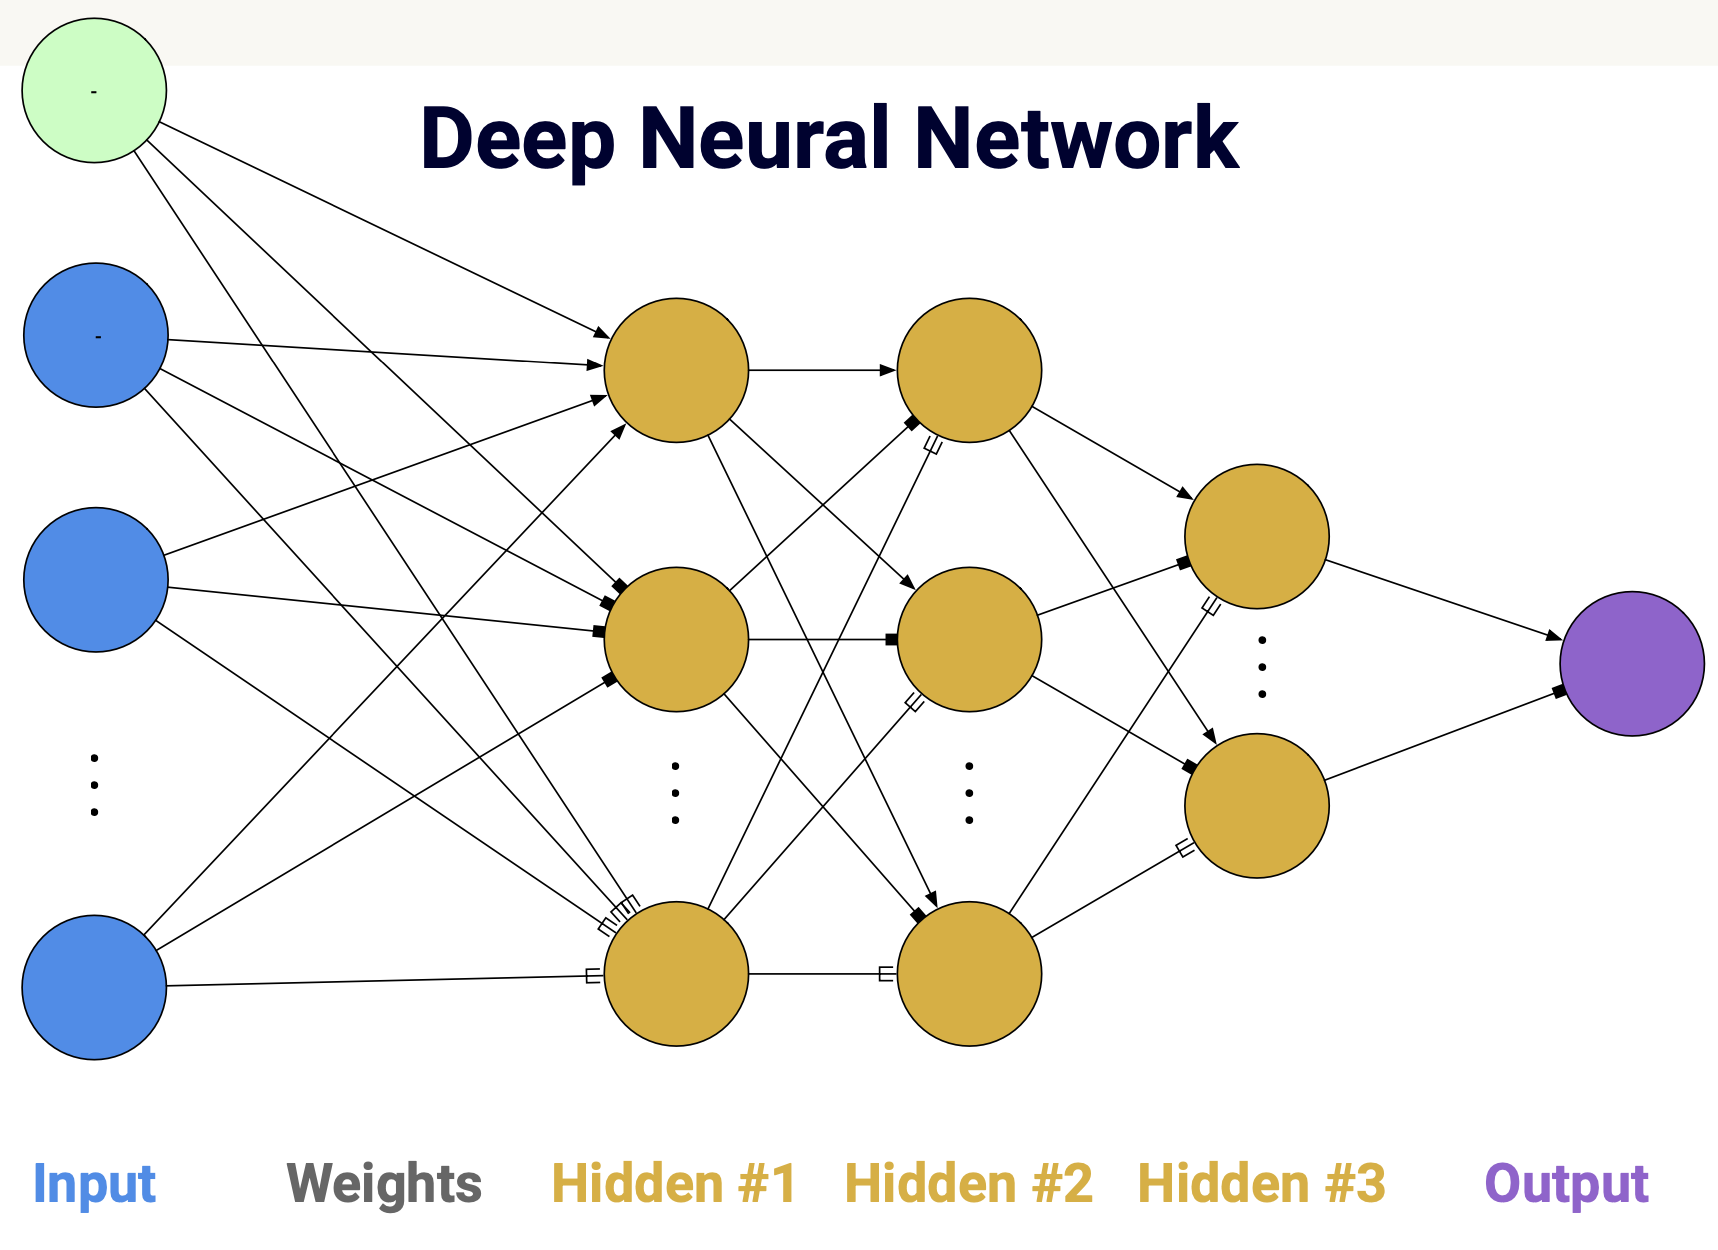
\includegraphics[scale=0.13]{deep.png}
    \caption{Deep Neural Network}
    \label{}
\end{figure}\end{center}
A deep neural network contains \textit{Input Layer}, \textit{Hidden Layer}, and \textit{Output Layer}.


\subsection{Universal Approximation Theorem}
Universal Approximation Theorem, in its lose form, states that a \textbf{feed-forward network} with a \textbf{single hidden layer} containing a finite number of neurons \textbf{can approximate any continuous function}. (Which is also equivalent to having a nonpolynomial activation function)
\begin{theorem}[Universal approximation theorem]
    Fix a continuous function $\sigma: \mathbb{R} \rightarrow \mathbb{R}$ (activation function) and positive integers $d, D\in \mathbb{Z}^+$. The function $\sigma$ is \underline{not a polynomial} $\Leftrightarrow$ for every continuous function $f: \mathbb{R}^d \rightarrow \mathbb{R}^D$ (target function), every compact subset $K$ of $\mathbb{R}^d$, and every $\epsilon>0$ there exists a continuous function $f_\epsilon: \mathbb{R}^d \rightarrow \mathbb{R}^D$ (the layer output) with representation $$f_\epsilon=W_2 \circ \sigma \circ W_1$$
    where $W_2, W_1$ are composable affine maps and o denotes component-wise composition, such that the approximation bound $$\sup _{x \in K}\left\|f(x)-f_\epsilon(x)\right\|<\varepsilon$$
    holds for any $\epsilon$ arbitrarily small (distance from $f$ to $f_\epsilon$ can be infinitely small).
\end{theorem}

\begin{center}\begin{figure}[htbp]
    \centering
    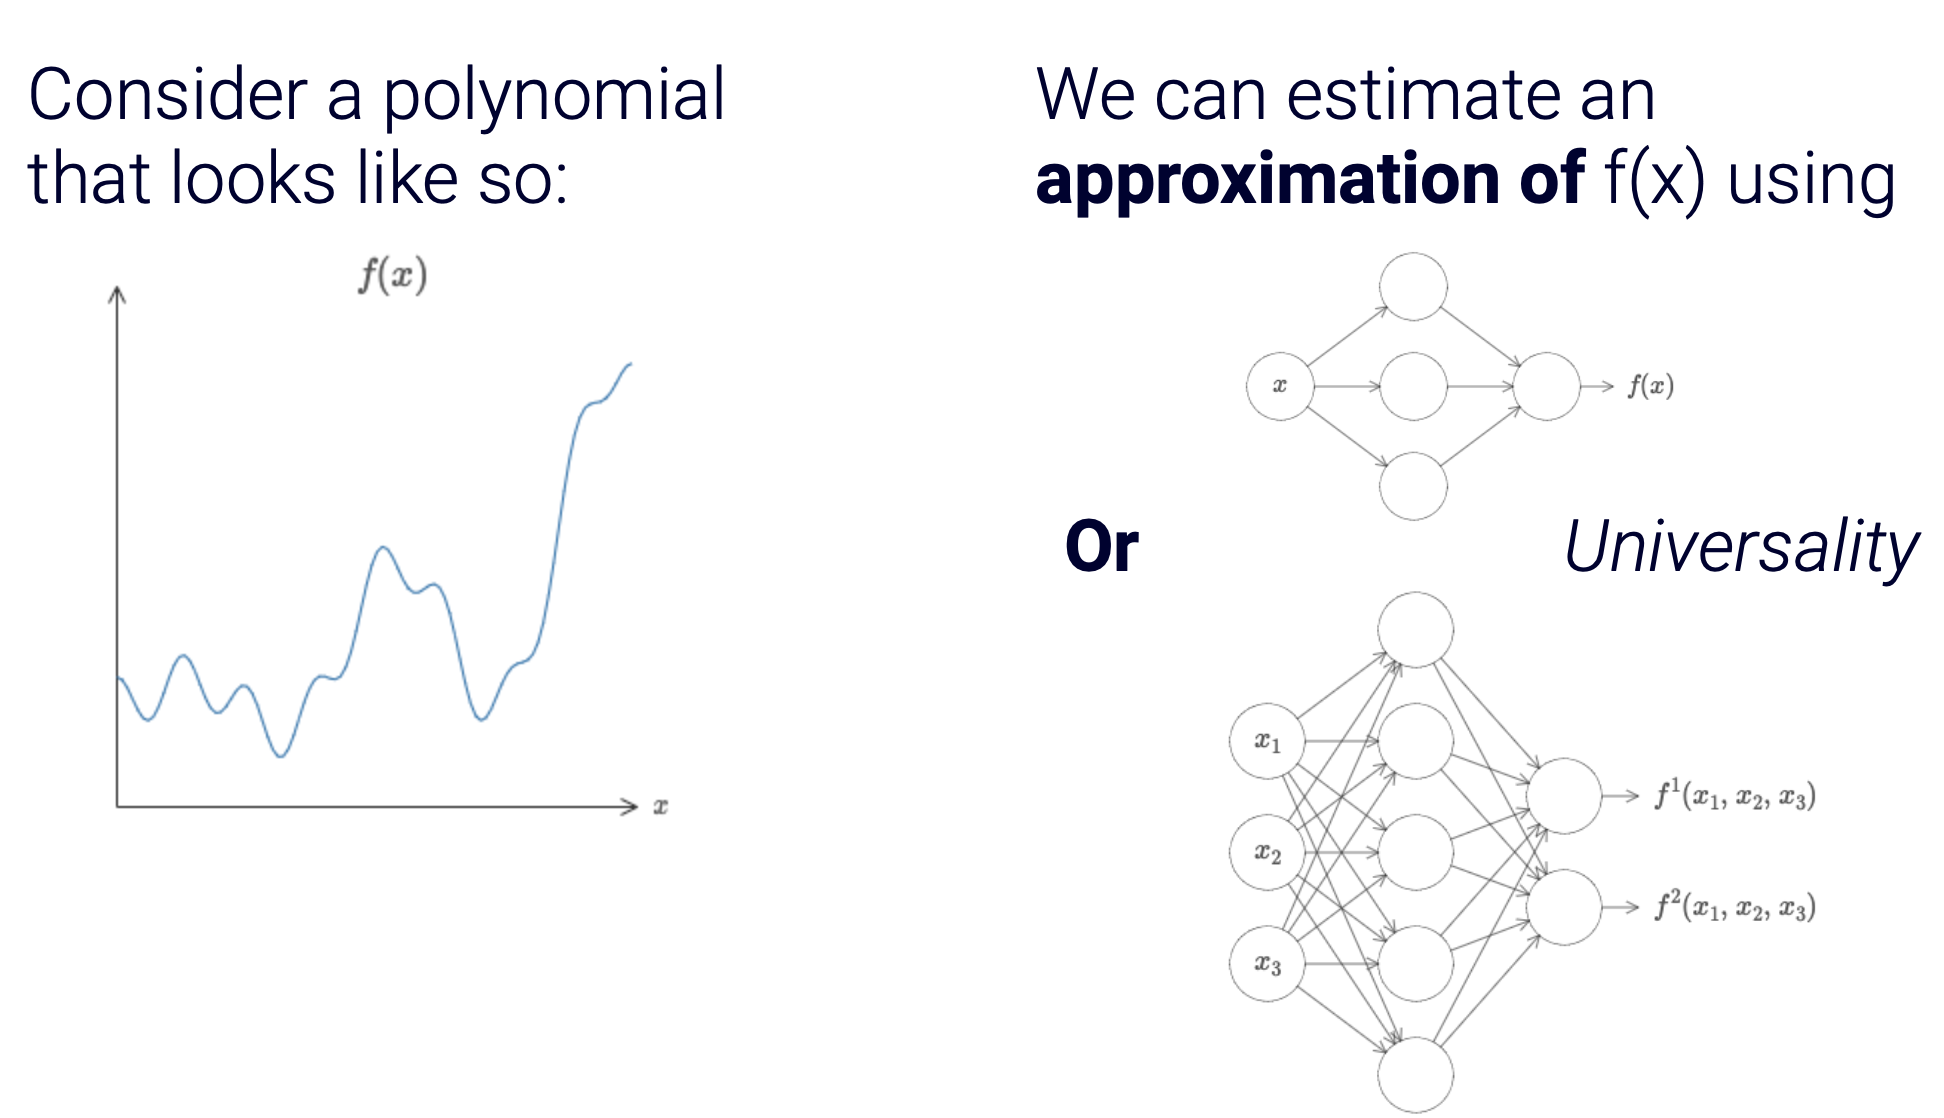
\includegraphics[scale=0.2]{UAT.png}
    \caption{Universal Approximation Theorem}
    \label{}
\end{figure}\end{center}

\section{ Mini-batch Optimization}
\subsection{Stochastic Gradient Descent (SGD) and Batch Gradient Descent (BGD)}
\textbf{Stochastic Gradient Descent (SGD)}
\begin{enumerate}
    \item Start with a random guess.
    \item For $n$ epochs:
    \begin{enumerate}[1)]
        \item Reorder data
        \item Retrieve an observation $i=1,2,...$ one by one in reordered data:
        \begin{enumerate}[(1)]
            \item Compute gradient on single data point $i$: $\frac{\partial J_i(W)}{\partial W}$
            \item Update parameters:
            $W=W-\alpha \frac{\partial J_i(W)}{\partial W}$
        \end{enumerate}
    \end{enumerate}
    \item Output parameters
\end{enumerate}
\textbf{Note:} "On-line"/"Stochastic" \textbf{Single} Observation Updates

\textbf{Batch Gradient Descent (BGD)}
\begin{enumerate}
    \item Start with a random guess.
    \item For $n$ epochs:
    \begin{enumerate}[1)]
        \item Compute gradients on
        \textbf{all the data}: $\frac{\partial J(W)}{\partial W}$
        \item Update parameters:
        $W=W-\alpha \frac{\partial J(W)}{\partial W}$
    \end{enumerate}
    \item Output parameters
\end{enumerate}
\textbf{Note:} \textbf{All} data used in update
\begin{center}\begin{figure}[htbp]
    \centering
    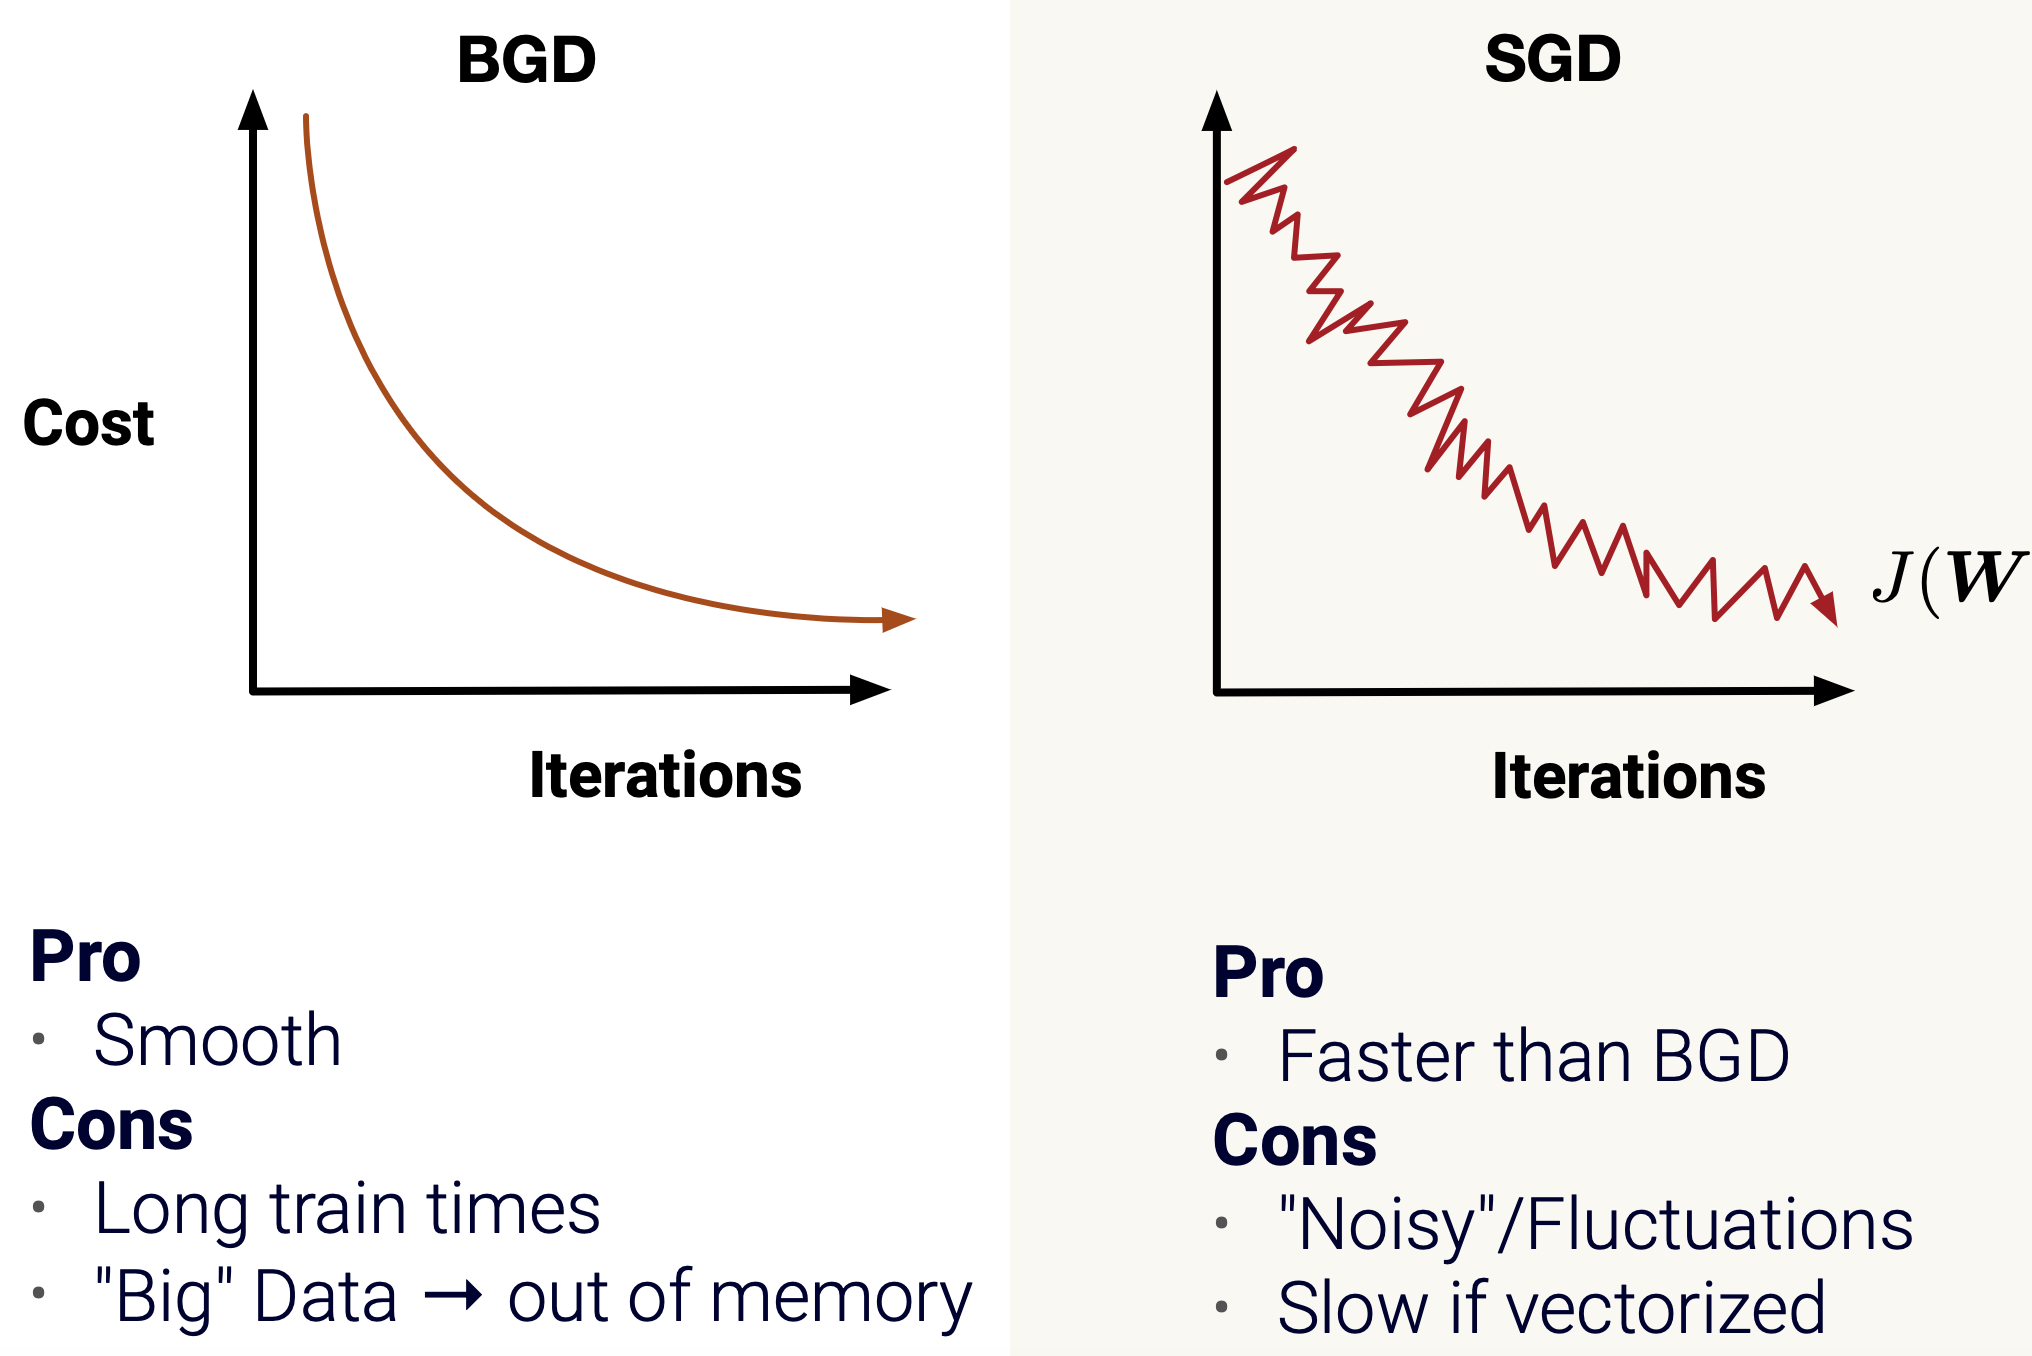
\includegraphics[scale=0.1]{BGDandSGD.png}
    \caption{BGD and SGD}
    \label{}
\end{figure}\end{center}

\subsection{Mini-Batch Gradient Descent (MBGD)}
We want a middle ground between SGD and BGD.

\textbf{Mini-Batch Gradient Descent (MBGD)}
\begin{enumerate}
    \item Start with a random guess.
    \item For $n$ epochs:
    \begin{enumerate}[1)]
        \item Reorder data and retrieve a subet of reordered data with size $b$ (batch size)
        \item Compute gradient on subset: $\frac{\partial J(W)}{\partial W}$
        \item Update parameters:
        $W=W-\alpha \frac{\partial J(W)}{\partial W}$
    \end{enumerate}
    \item Output parameters
\end{enumerate}
If $b=n$, the algorithm is exactly BGD; If $b=1$, the algorithm is exactly SGD.
\begin{center}\begin{figure}[htbp]
    \centering
    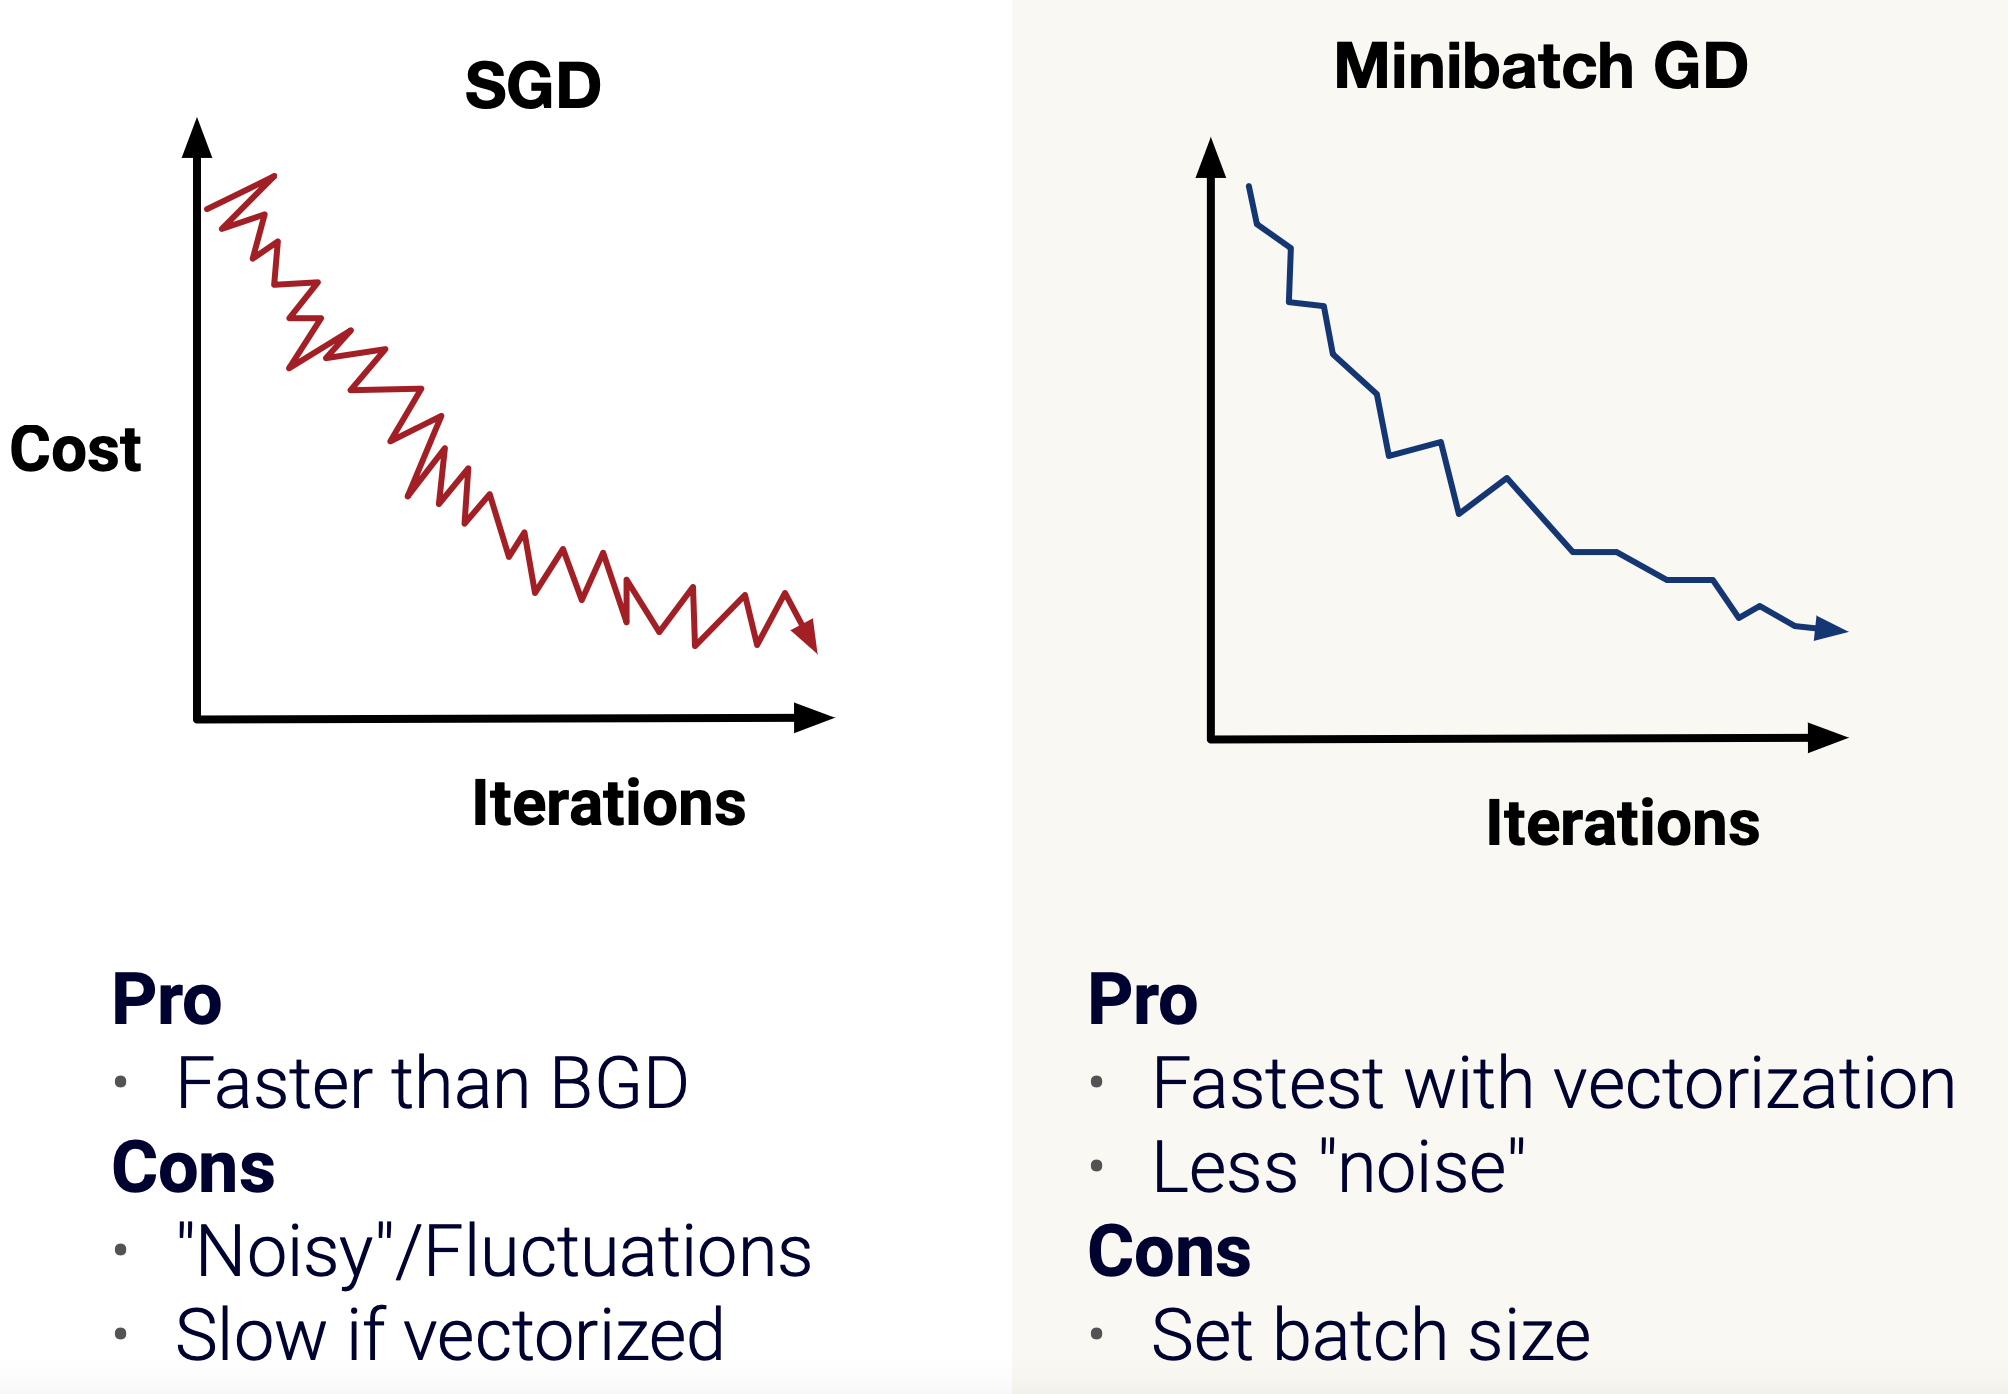
\includegraphics[scale=0.1]{SGDandMBGD.png}
    \caption{SGD and MBGD}
    \label{}
\end{figure}\end{center}

\begin{center}\begin{figure}[htbp]
    \centering
    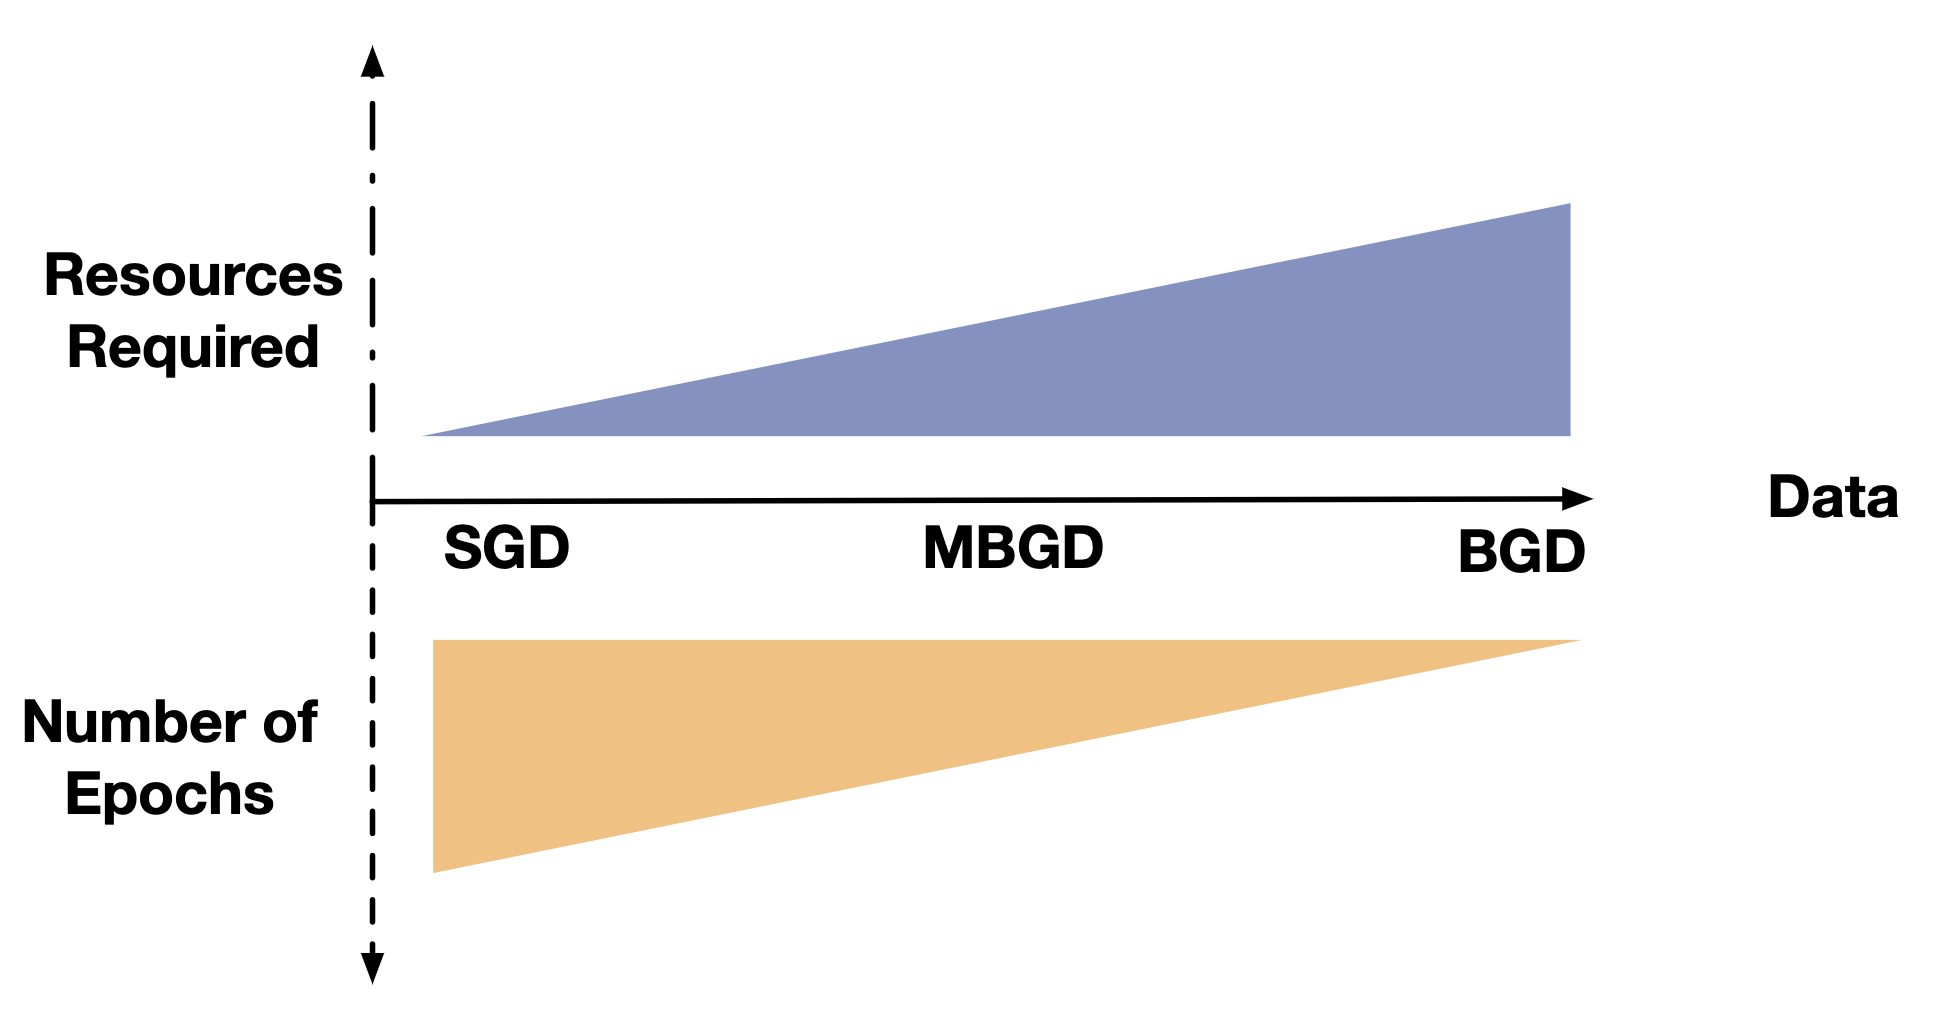
\includegraphics[scale=0.1]{resource.png}
    \caption{Comparison of Approaches}
    \label{}
\end{figure}\end{center}

\section{Weight Initialization}
\subsection{Xavier Initialization}
Normal distribution with a scale variance by weights. Used on layers where either $TanH$ or $Sigmoid$ is present.
\begin{center}
    Initialize weights for layer $l$ with: $W^{[l]}=W^{[l]}\sqrt{\frac{1}{n^{[l-1]}}}$
\end{center}
where $n^{[l-1]}$ is the number of weights in the last layer. Each weight is sampled by $W_{j,i}^{[l]}\sim \mathcal{N}(0,1)$

\subsection{He Activation}
Weight initialization for $ReLU$-powered network.
\begin{center}
    Initialize weights for layer $l$ with: $W^{[l]}=W^{[l]}\sqrt{\frac{2}{n^{[l-1]}}}$
\end{center}
where $n^{[l-1]}$ is the number of weights in the last layer. Each weight is sampled by $W_{j,i}^{[l]}\sim \mathcal{N}(0,1)$


\chapter{Adaptive Optimization}
\section{Exponentially Weighted Moving Averages}
How can we get an average across time?
\begin{enumerate}
    \item (Simple) (weighted) Moving Average ((S)MA): $$\bar{x}_{MA}=\frac{x_m+x_{m-1}+\cdots+x_{m-(n-1)}}{n}=\frac{1}{n}\sum_{i=0}^{n-1}x_{m-i}$$
    \item Exponentially (weighted) Moving Averages (EMA):
    \begin{equation}
        \begin{aligned}
            {EMA}_{t}=\left\{\begin{matrix}
                Y_1,&t=1\\
                \beta \cdot Y_t+(1-\beta)\cdot {EMA}_{t-1},&t>1
            \end{matrix}\right.
        \end{aligned}
        \nonumber
    \end{equation}
\end{enumerate}
$EMA$ is quicker to react: focuses more on recent events; $SMA$ is slower to react: focuses on long series events.

\section{Adaptive Learning Rates}
\textit{Adaptive Learning Rate} is a change to the learning rate while training a model to reduce the training time and improve output
\subsection{Momentum}
For a gradient descent with form:
\begin{equation}
    \begin{aligned}
        \theta_{t+1}:=\theta_t-v_t
    \end{aligned}
    \nonumber
\end{equation}
where $v_t$ is the \textbf{velocity} which is amplified gradient speed.
\begin{enumerate}
    \item \textbf{SGD:} $$v_t=\alpha \nabla_\theta J(\theta_t)$$
    \item \textbf{SGD + Momentum:} $$v_t=\rho v_{t-1}+\alpha \nabla_\theta J(\theta_t)$$
    where $\rho$ is the \textbf{friction or momentum} which dampens the amount of the previous gradient included. Default: $0.9$ for $\sim 10$ gradients.
\end{enumerate}
With momentum, the learning rate is \textbf{decreased} if gradient direction changes and \textbf{increased} if gradient direction stays on same path.

\subsection{Root Mean Square Propagation (RMSProp)}
Decrease learning rate by EMA using squared gradient.
\begin{equation}
    \begin{aligned}
        g_0&=0\quad (\text{Initial "gain"})\\
        g_t&=\alpha g_{t-1}+(1-\alpha) \nabla_\theta J(\theta_t)^2\quad (\text{MA over gradient squared})\\
        \theta_t:&=\theta_{t-1}-\frac{\varepsilon}{\sqrt{g_t}+1\times 10^{-5}}v_t\quad (1\times 10^{-5} \text{ is used to avoid division by $0$})\\
    \end{aligned}
    \nonumber
\end{equation}

\subsection{Adaptive Moment Estimation (ADAM)}
Merges the momentum and RMSProp paradigms.\\
Novelty is a bias correction of 1st/2nd moments.\\
Focus is on learning rate annealing (start fast, decrease).
\begin{enumerate}[(1)]
    \item \textbf{Initial:} $v_0=0,g_t=0$.
    \item \textbf{Momentum-variant:} $v_t=\beta_1 v_{t-1}+(1-\beta_1) \nabla_\theta J(\theta_t)$
    \item \textbf{RMSProp:} $g_t=\beta_2 g_{t-1}+(1-\beta_2) \nabla_\theta J(\theta_t)^2$
    \item \textbf{Bias Correction:} $v'_t=\frac{v_t}{1-\beta_1^t}$, $g'_t=\frac{g_t}{1-\beta_2^t}$ (where $\beta_i^t$ is the $t^{\textnormal{th}}$ power of $\beta_i$)
    \item \textbf{RMSProp + Momentum:} $\theta_t:=\theta_{t-1}-\frac{\varepsilon}{\sqrt{g'_t}+1\times 10^{-5}}v'_t$
\end{enumerate}
\textit{Pytorch Code}
\begin{lstlisting}[language=Python]
    torch.optim.Adam(params, lr=0.001, betas=(0.9, 0.999), eps=1e-08,
                    weight_decay=0, amsgrad=False, *, foreach=None,
                    maximize=False, capturable=False,
                    differentiable=False, fused=False)
\end{lstlisting}
\textit{Pseudocode}
\begin{center}\begin{figure}[htbp]
    \centering
    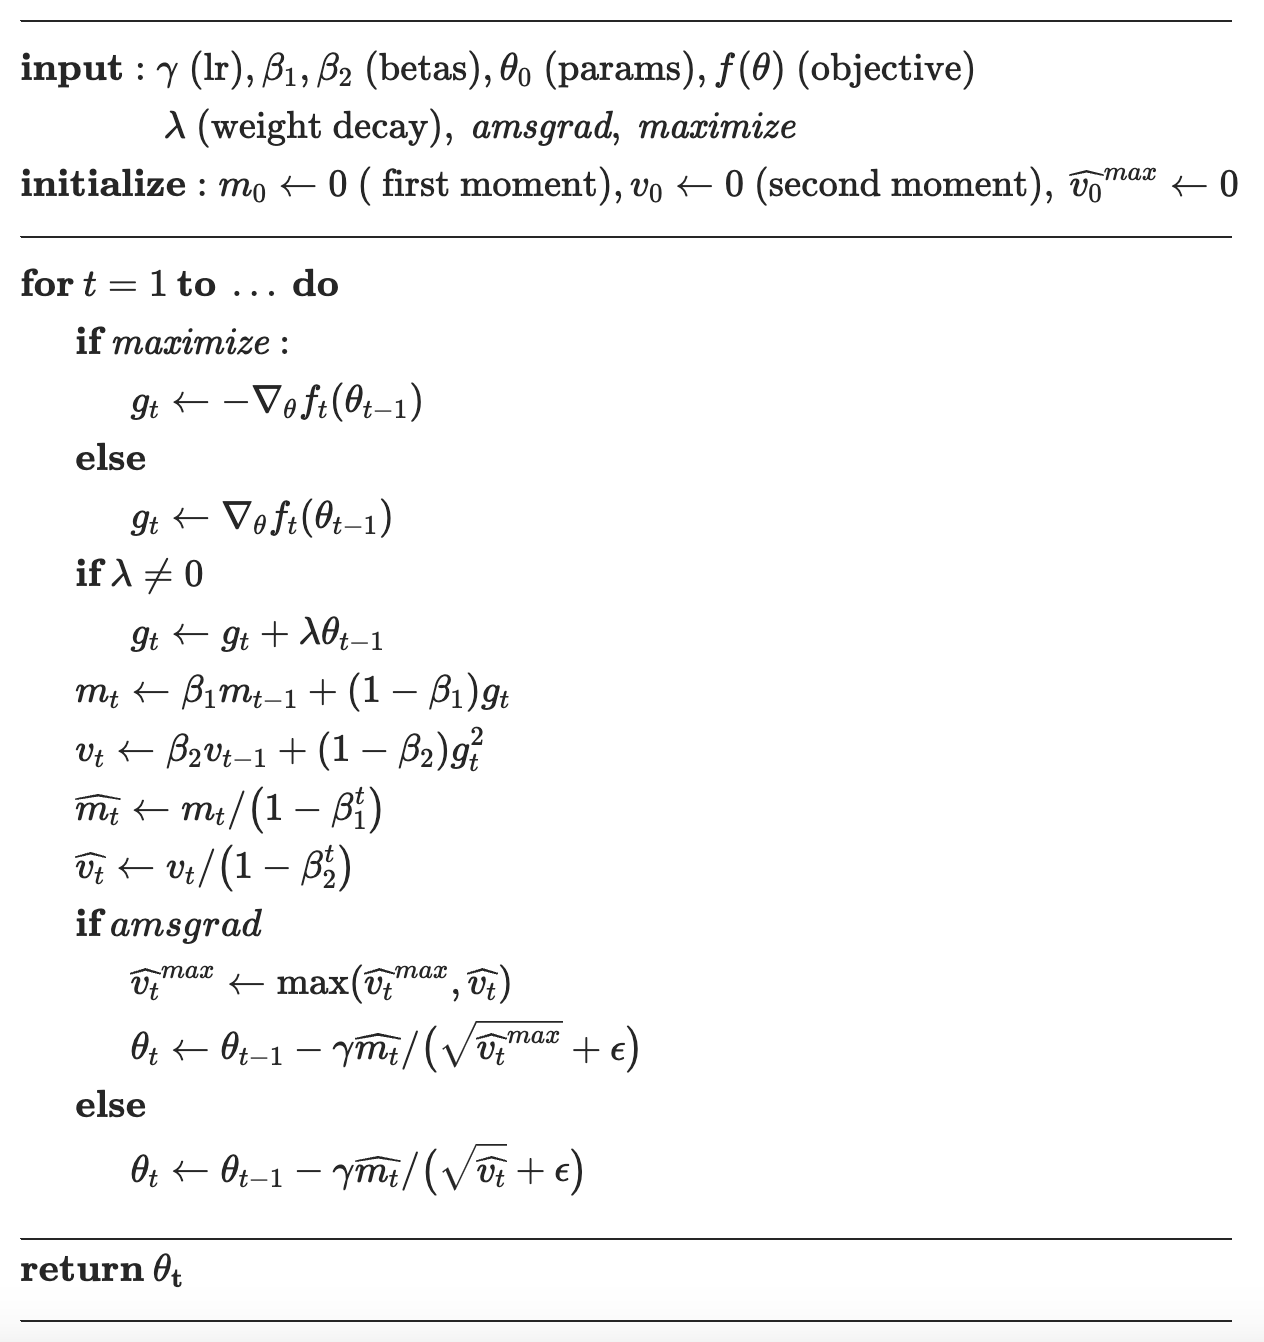
\includegraphics[scale=0.25]{Adam_code.png}
    \caption{Pseudocode of ADAM}
    \label{}
\end{figure}\end{center}


\chapter{Convolutional Neural Network (CNN)}
\section{Convolution and Cross-correlation}
Cross-correlation and convolution are both operations applied to images. Cross-correlation means sliding a kernel (filter) across an image. Convolution means sliding a flipped kernel across an image. \textbf{Most convolutional neural networks in machine learning libraries are actually implemented using cross-correlation}, but it doesn't change the results in practice because if convolution were used instead, the same weight values would be learned in a flipped orientation.

We have some \textit{source pixels}, we use a \textit{convolution kernel} (filter) to process the \textit{source pixels}. The output is \textit{destination pixels}.

Given the \textit{source pixels} $\{\textbf{Image}(x,y):x\in [-d_X,d_X],y\in [-d_Y,d_Y]\}$ and \textit{convolution kernel} (filter) $\{K(i,j):i,j\in[-d,d]\}$. $n_X=2d_X+1,n_Y=2d_Y+1$ are image dimension, $f=2d+1$ is the filter dimension. We can generate destination pixels in $(n_X-f+1)\times (n_Y-f+1) = (n_X-2d)\times (n_Y-2d)$

For $x\in [d+1,n_X-d],y\in [d+1,n_Y-d]$
\begin{enumerate}
    \item \textbf{Convolution:}
    \begin{equation}
        \begin{aligned}
            \textbf{CONV}(x,y)=\sum_{i=-d}^d\sum_{j=-d}^d \textbf{Image}(x-i,y-j)K(i,j)
        \end{aligned}
        \nonumber
    \end{equation}
    \item \textbf{Cross-Correlation:}
    \begin{equation}
        \begin{aligned}
            \textbf{CrossCorrelation}(x,y)=\sum_{i=-d}^d\sum_{j=-d}^d \textbf{Image}(x+i,y+j)K(i,j)
        \end{aligned}
        \nonumber
    \end{equation}
\end{enumerate}

\begin{center}\begin{figure}[htbp]
    \centering
    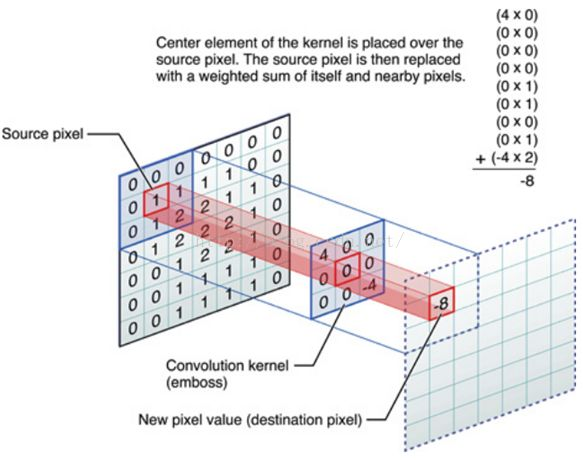
\includegraphics[scale=0.5]{convolution.jpeg}
    \caption{Convolution Used in CNN (actually cross-correlation)}
    \label{}
\end{figure}\end{center}

\subsection*{Kernel}
\begin{enumerate}
    \item \textbf{Edge Detection:} vertical $\begin{bmatrix}
        1&0&-1\\
        1&0&-1\\
        1&0&-1
    \end{bmatrix}$; horizontal $\begin{bmatrix}
        1&1&1\\
        0&0&0\\
        -1&-1&-1
    \end{bmatrix}$
    \item {Blur Pixel:} $\frac{1}{9}\begin{bmatrix}
        1&1&1\\
        1&1&1\\
        1&1&1
    \end{bmatrix}$; 
    {Sharpen:} $\begin{bmatrix}
        0&0&0\\
        0&2&0\\
        0&0&0
    \end{bmatrix}$; 
    {Identity:} $\begin{bmatrix}
        0&0&0\\
        0&1&0\\
        0&0&0
    \end{bmatrix}$; 
    {Shift Pixel:} $\begin{bmatrix}
        0&0&0\\
        1&0&0\\
        0&0&0
    \end{bmatrix}$
\end{enumerate}



\section{Padding (cover the border)}
\begin{definition}
    \underline{Padding} refers to the extension of the input image by adding a border of pixels the image.
\end{definition}
\begin{center}\begin{figure}[htbp]
    \centering
    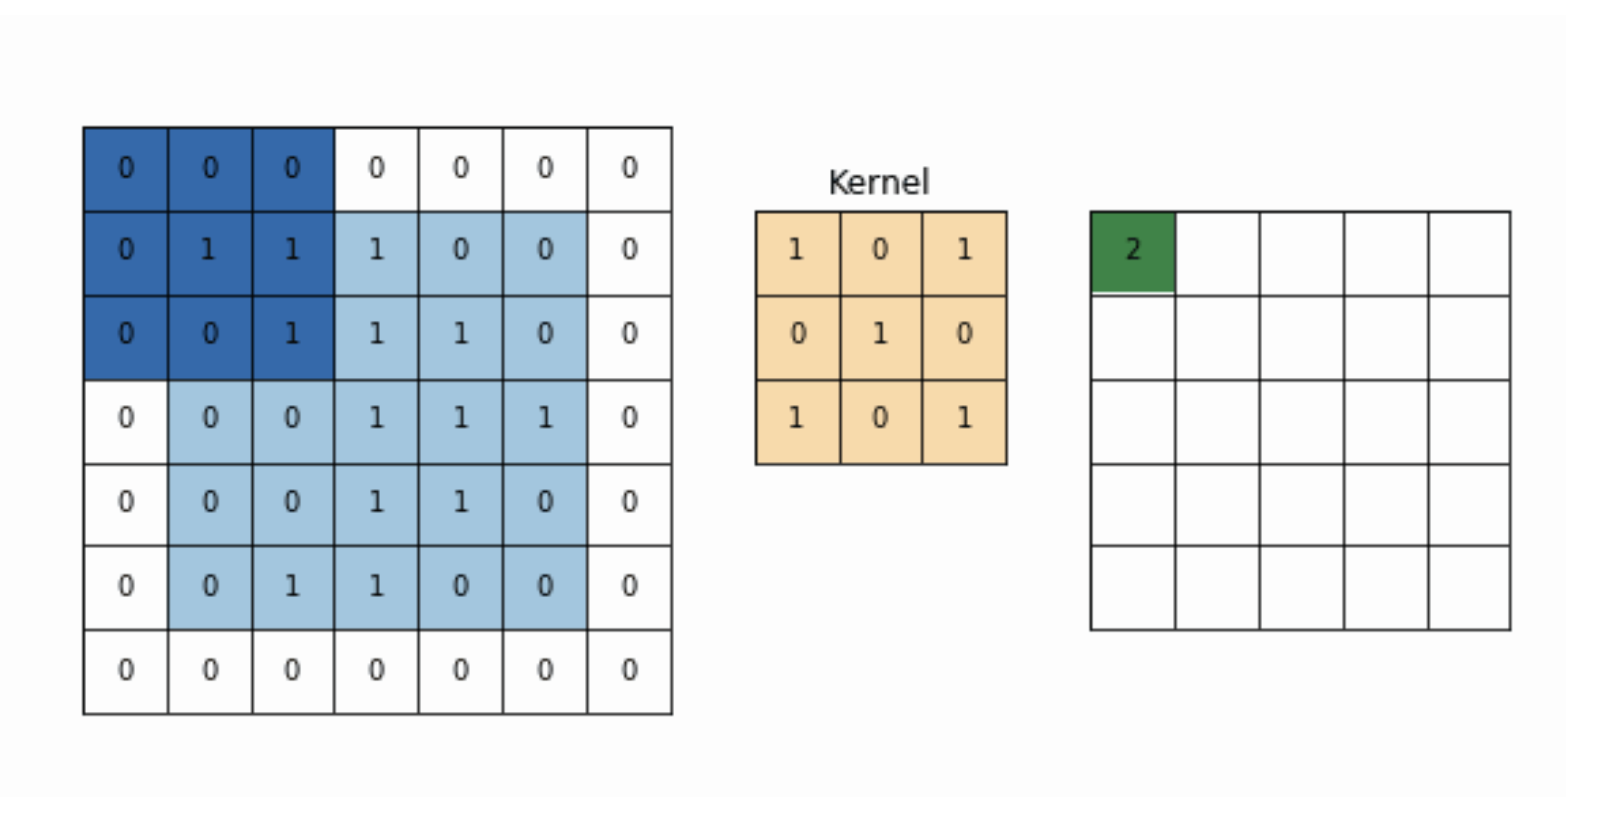
\includegraphics[scale=0.15]{Padding.png}
    \caption{Padding: $p=1$}
    \label{}
\end{figure}\end{center}
For image $n\times n$ with filter $f\times f$ and padding $p$, the output has dimension
\begin{equation}
    \begin{aligned}
        (n+2p-f +1)\times (n+2p-f +1)
    \end{aligned}
    \nonumber
\end{equation}
In order for the output dimensions to be equivalent to the image dimension the padding value must be $p=\frac{f-1}{2}$

\section{Stride}
\begin{definition}
    \underline{Stride} refers to the sliding distance of the filter/kernel over spatial locations.
\end{definition}
The default stride or strides in two dimensions is (1,1) for the height and the width movement.

For example, the stride can be changed to (2,2). This has the effect of moving the filter two pixels right for each horizontal movement of the filter and two pixels down for each vertical movement of the filter when creating the feature map.

The new dimension of the output would be
\begin{equation}
    \begin{aligned}
        \left\lfloor \frac{n_X+2p-f}{s}+1\right\rfloor\times\left\lfloor \frac{n_Y+2p-f}{s}+1\right\rfloor
    \end{aligned}
    \nonumber
\end{equation}

\section{Other Layer Types}
\subsection{Pooling}
\begin{definition}
    \underline{Pooling} refers to the process of downsampling features by aggregating values at places in the feature map.
\end{definition}
\begin{center}\begin{figure}[htbp]
    \centering
    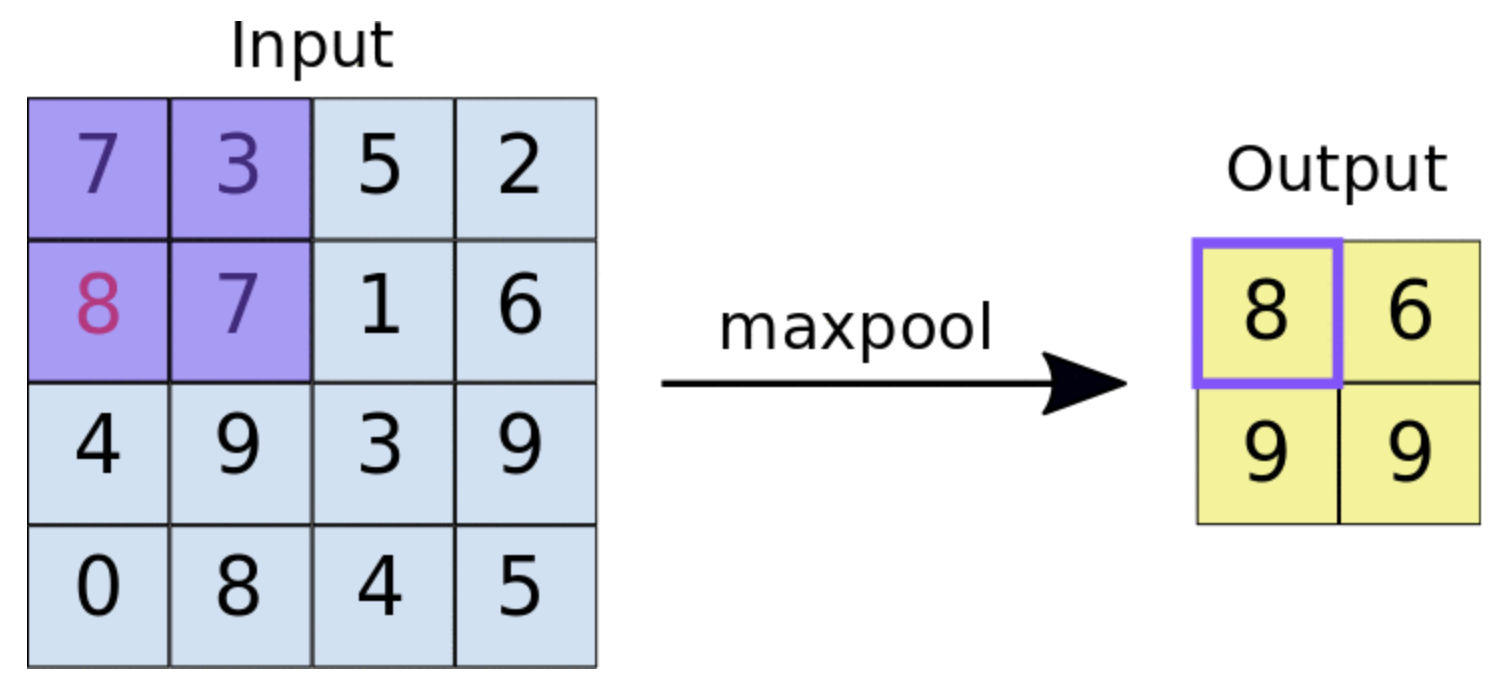
\includegraphics[scale=0.1]{maxpool.png}
    \caption{Example: maxpool}
    \label{}
\end{figure}\end{center}

\subsection{Unpooling}
\begin{definition}
    \underline{Unpooling} refers to the process of upsampling features by recreating the dimensions of feature map pooled and placing the pooled values into their original location.
\end{definition}
\begin{center}\begin{figure}[htbp]
    \centering
    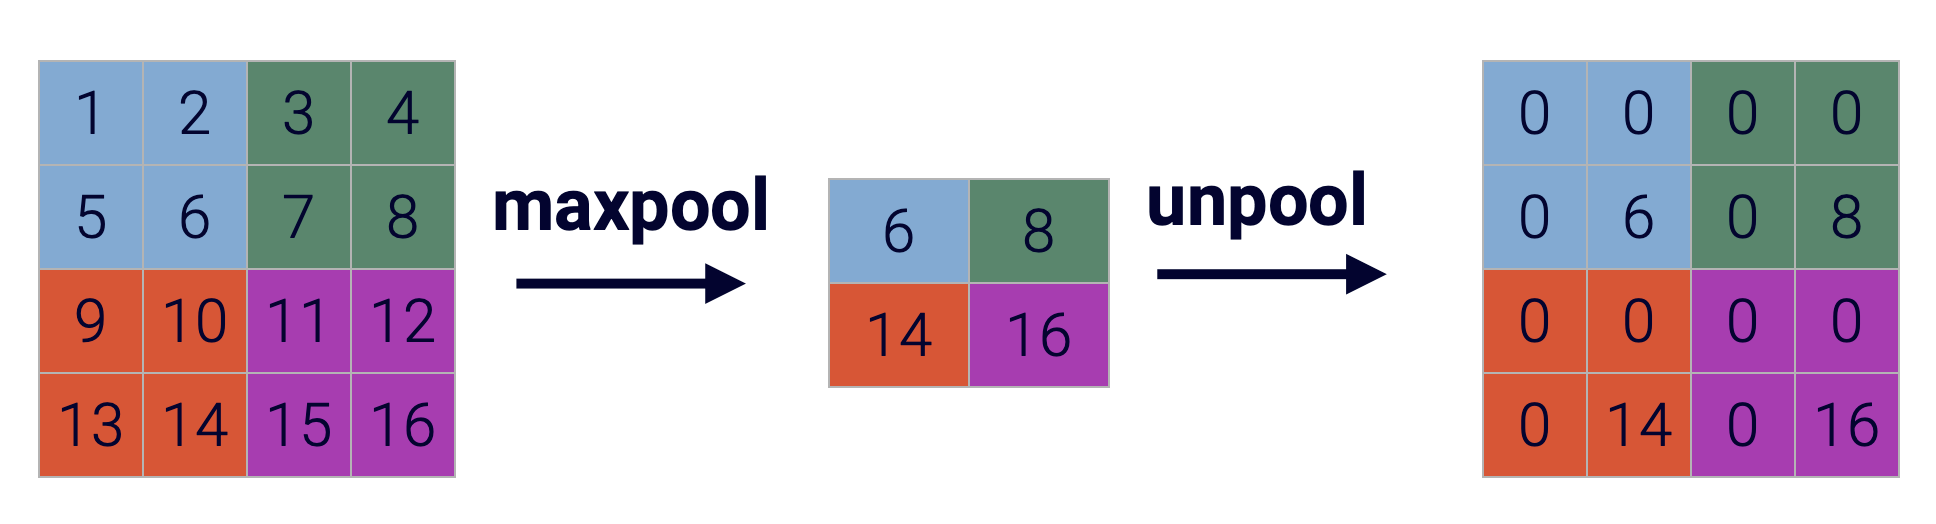
\includegraphics[scale=0.1]{unpool.png}
    \caption{Example: maxpool+unpool}
    \label{}
\end{figure}\end{center}

\section{3D Convolution}
\begin{center}\begin{figure}[htbp]
    \centering
    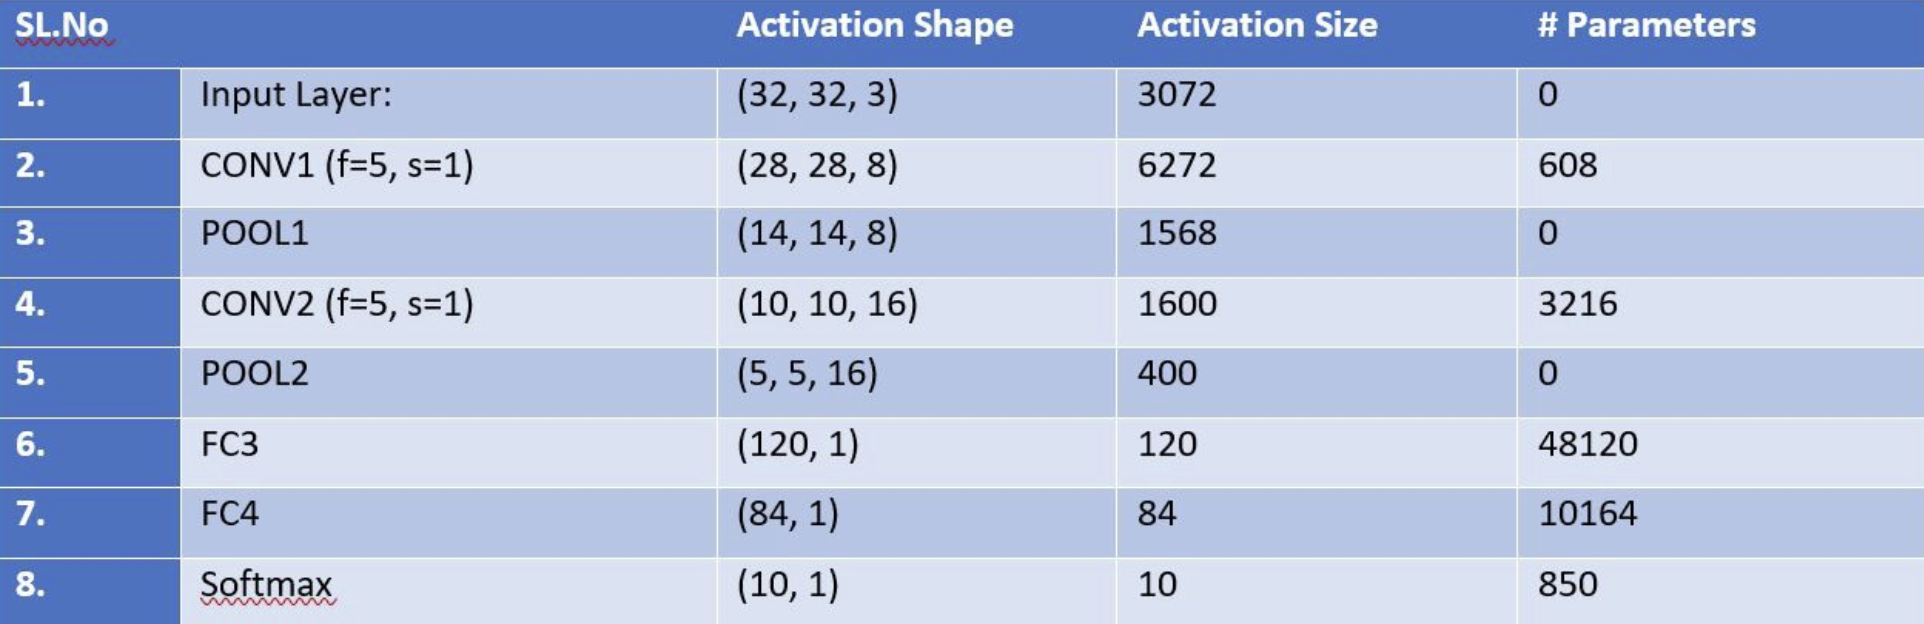
\includegraphics[scale=0.2]{3DConv.png}
    \caption{3D Convolution}
    \label{}
\end{figure}\end{center}
Note the default filter has dimension $f\times f\times n'$ ($n'$ is the number of filters in the previous layer)
\subsection*{Parameters Computing:}
\begin{enumerate}
    \item \textbf{CONV layer:} (shape of width of the filter * shape of height of the filter * number of filters in the previous layer+1)*number of filters\\
    (added 1 because of the bias term for each filter.)
    $$(5\times 5\times 3+1)\times 8=608$$
    \item \textbf{Fully Connected Layer (FC):} (current layer neurons number * previous layer neurons number)+1* current layer neurons number
    $$120\times 400+ 1\times 120=48120$$
\end{enumerate}






\chapter{Generative model}
\section{Autoencoders}
\textbf{Definition:} \textit{Self-supervised learning (SSL)} is a machine learning process where the model trains itself to learn one part of the input from another part of the input. It is a technique similar in scope to how humans learn to classify objects. SSL relies on unlabeled data to solve a task by splitting the task into at least two halves:
\begin{enumerate}
    \item A decomposition into pseudo-labels by withholding some training data (self-supervised task/pretext task); and,
    \item Reconstruction using either supervised or unsupervised learning.
\end{enumerate}
For example, in natural language processing, if we have a few words, using self-supervised learning we can complete the rest of the sentence. Similarly, in a video, we can predict past or future frames based on available video data.

\subsection{Basics}
\begin{definition}
    \textbf{Autoencoders} are designed to take the input data, say $x$, and, then, predict the very same input $x$! In other words, the network trains itself to imitate its input so that its output is the same.
\end{definition}
\begin{center}\begin{figure}[htbp]
    \centering
    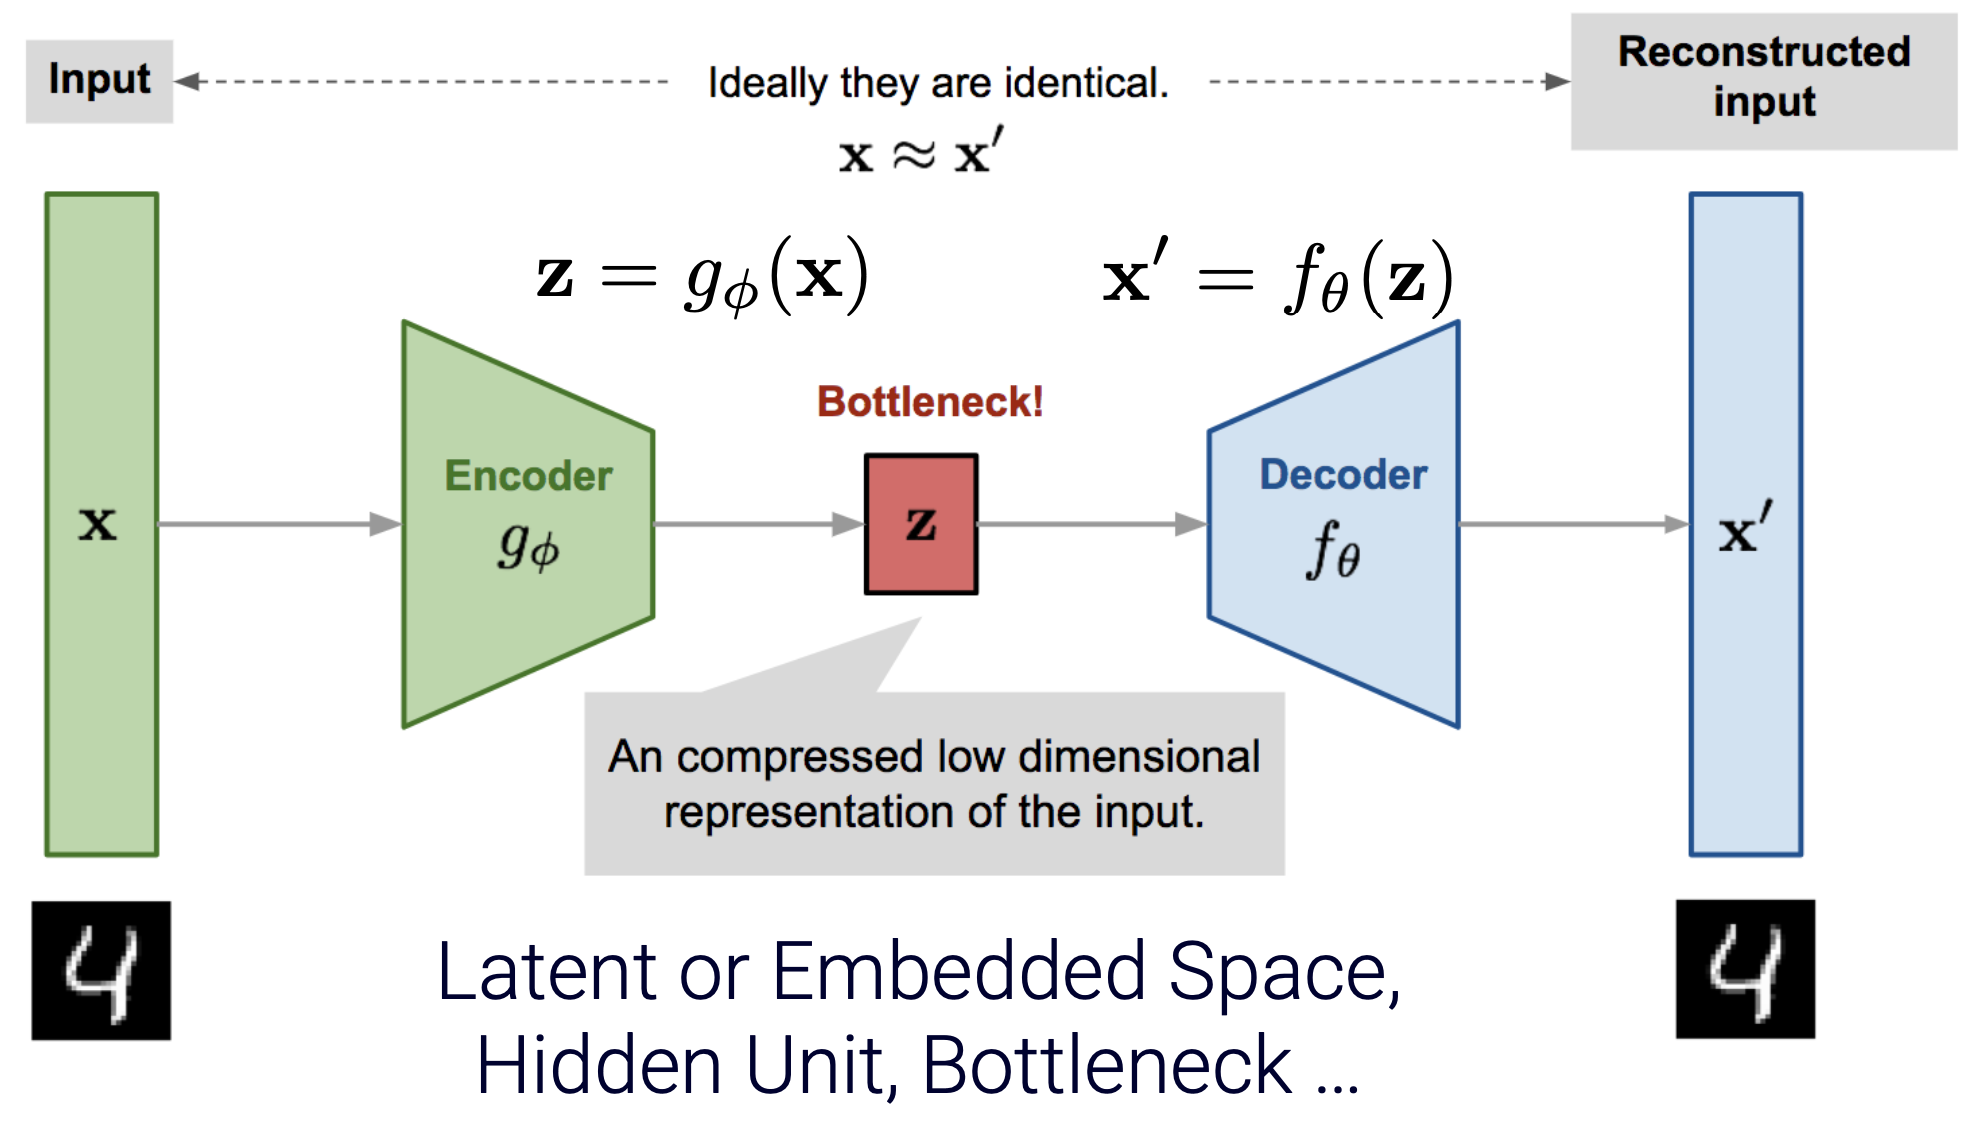
\includegraphics[scale=0.2]{Autoencoders.png}
    \caption{Autoencoders}
    \label{}
\end{figure}\end{center}
Undercomplete autoencoders are defined as having a bottleneck layer dimension that is less than that of the input. e.g. $$\text{dim}(z)<\text{dim}(x)$$
The lower dimention of bottleneck (hidden unit) avoids overfitting.

If the dimension is equal, the $x$ will be completely transformed into $x'$ which is often the same as the model learns nothing and may also be overfitted. Therefore, some other conditions are usually added to make the model only approximate its input, so that the model can really learn the hidden vector expression of the input samples and prevent overfitting.

\subsection{PCA and Autoencoders}

Principal Component Analysis (PCA) is using orthogonal basis to reduce dimensionality.
\begin{center}\begin{figure}[htbp]
    \centering
    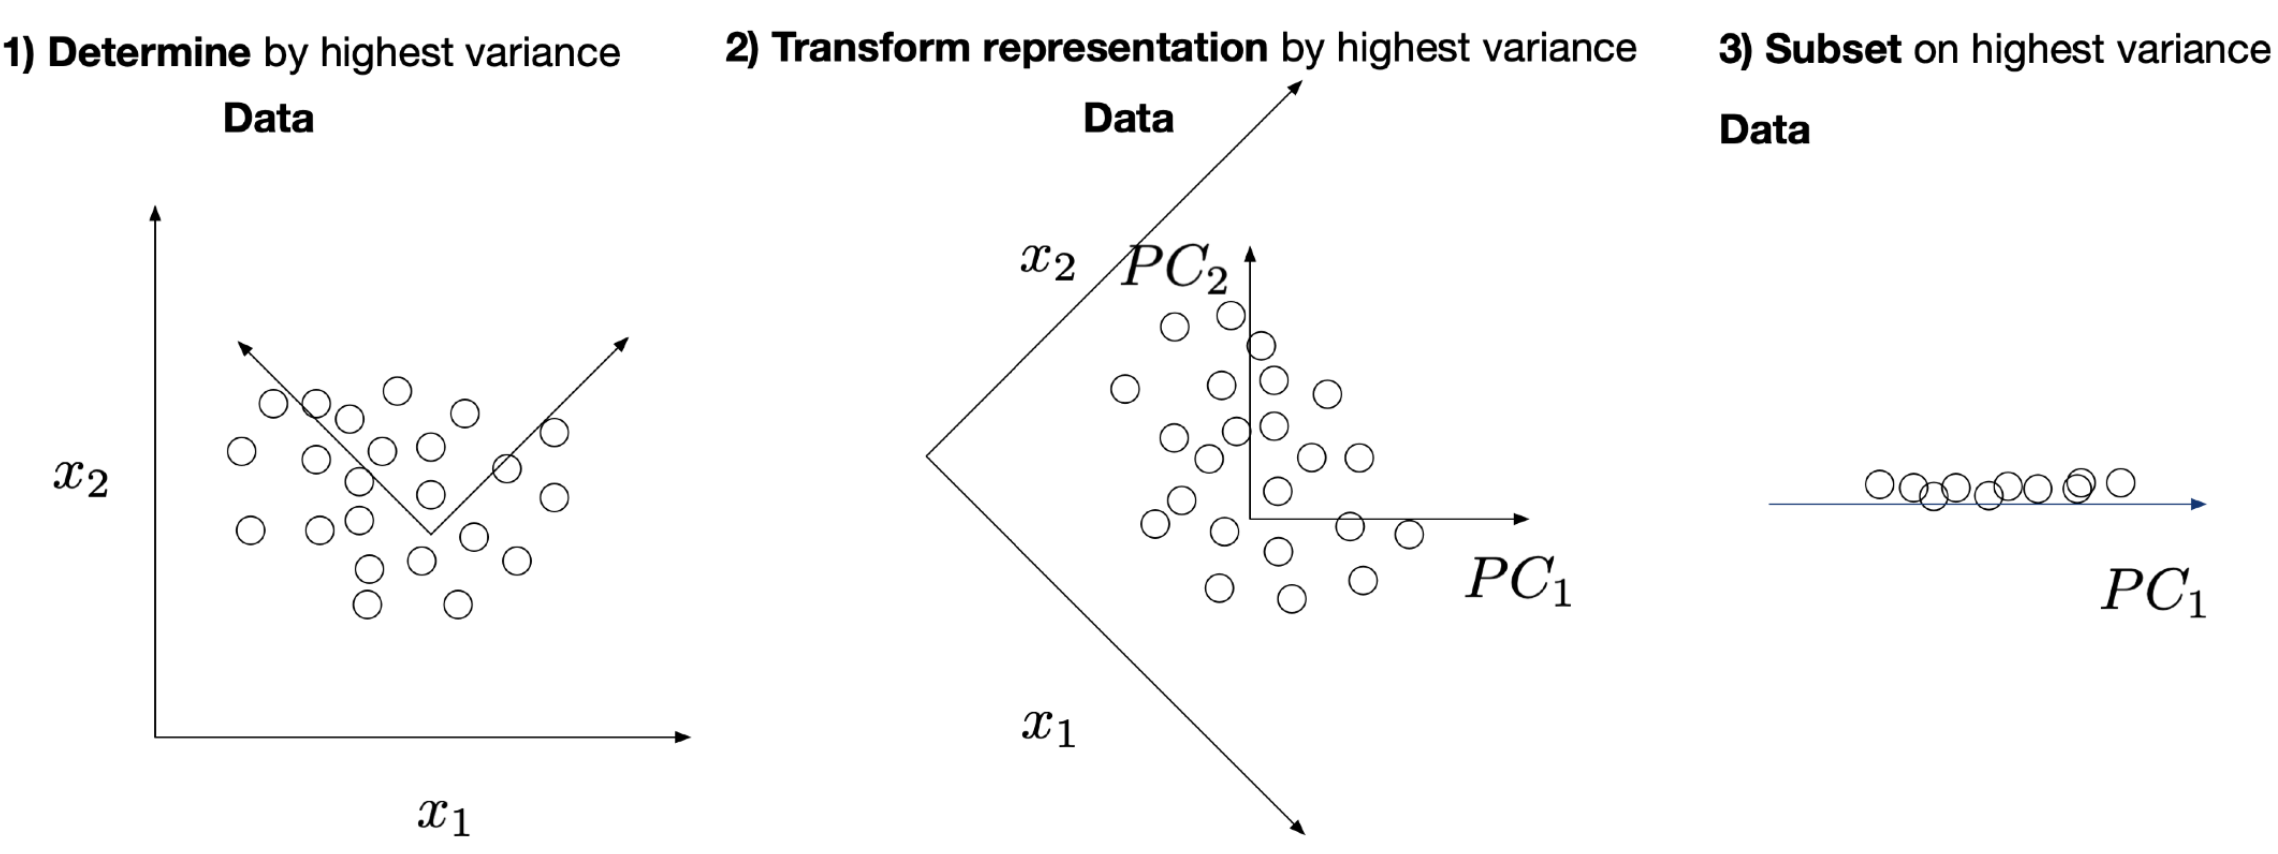
\includegraphics[scale=0.2]{PCA.png}
    \caption{Principal Component Analysis (PCA)}
    \label{}
\end{figure}\end{center}
Consider a single hidden layer linear autoencoder network with linear activations and MSE loss:
\begin{equation}
    \begin{aligned}
        \vec{z}&=W^{[1]}\vec{x}+\vec{b}^{[1]}\\
        \vec{x}'&=W^{[2]}\vec{z}+\vec{b}^{[2]}\\
        L(\vec{x},\vec{x}')&=\|\vec{x}-\vec{x}'\|^2_2
    \end{aligned}
    \nonumber
\end{equation}
If we have the ${dim}(m) < {dim}(n)$, then the problem will be a PCA without an orthogonality restriction on the weights.

\textbf{Why bother with autoencoders if PCA exists?} Dimensional Reductions (Addressing curse of dimensionality)

- Rarely are we seeking to use an auto encoder for solely a dimension reduction.\\
- In such cases, we probably would be better off with:
\begin{enumerate}[$\bullet$]
    \item Principal Component Analysis (PCA): If linear and desire global structure under a deterministic algorithm.
    \item T-distributed stochastic neighbour embedding (t-SNE): If non-linear and desire local structure under a randomized algorithm with dense structures.
    \item Uniform Manifold Approximation and Projection (UMAP): If non-linear and desire local structure under a randomized algorithm with sparse structures.
\end{enumerate}

\subsection{Transposed Convolutions (upscale method)}
\textbf{Definition:} \textit{Transposed Convolutions}, \textit{uncov}, or \textit{fractionally striped convolution} is a technique to upscale the feature map so that it matches in dimension with the input feature map.\\
(Sometimes erroneously called "deconvolution".)
\begin{center}\begin{figure}[htbp]
    \centering
    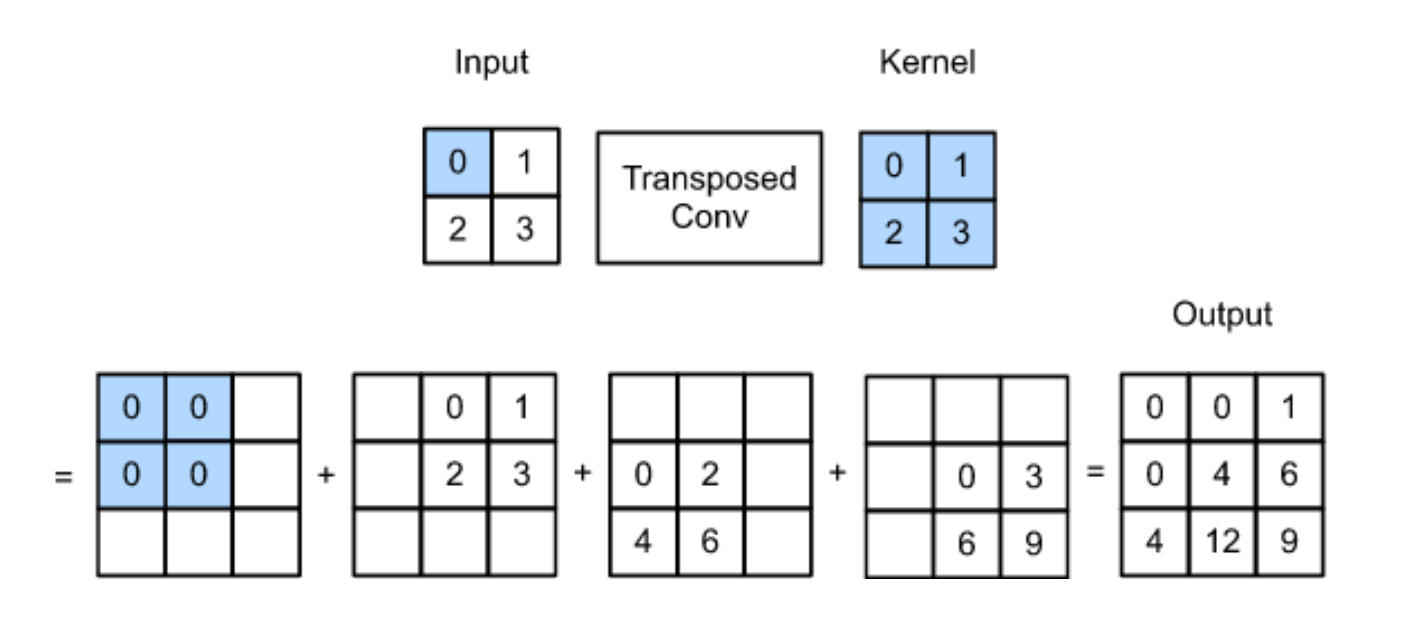
\includegraphics[scale=0.2]{Transposed Convolutions.png}
    \caption{Transposed Convolutions}
    \label{}
\end{figure}\end{center}
\subsection*{Comparison between Convolution and Transposed Convolution}
\begin{center}\begin{figure}[htbp]
    \centering
    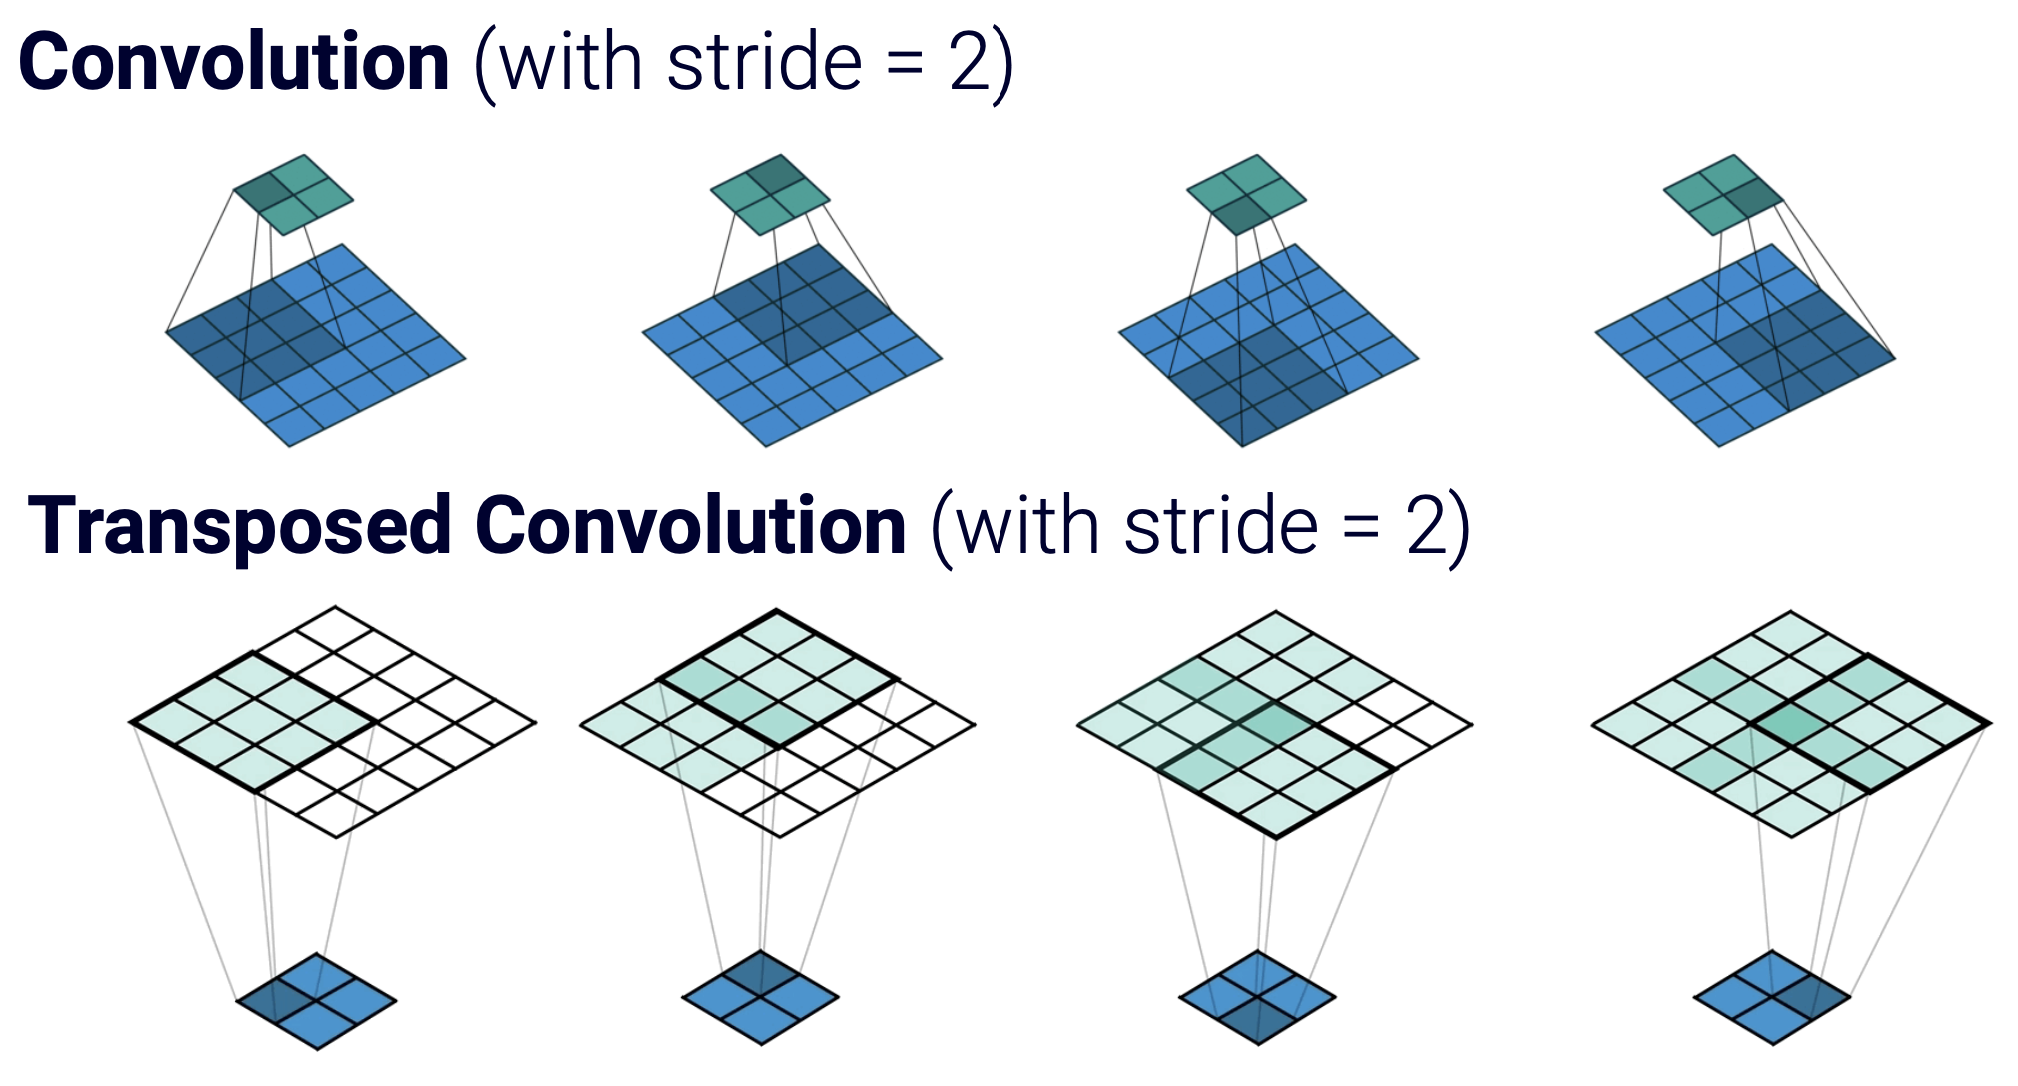
\includegraphics[scale=0.2]{Comparison_conv.png}
    \caption{Comparison}
    \label{}
\end{figure}\end{center}
\subsection*{Transposed Convolution with Stride}
\begin{center}\begin{figure}[htbp]
    \centering
    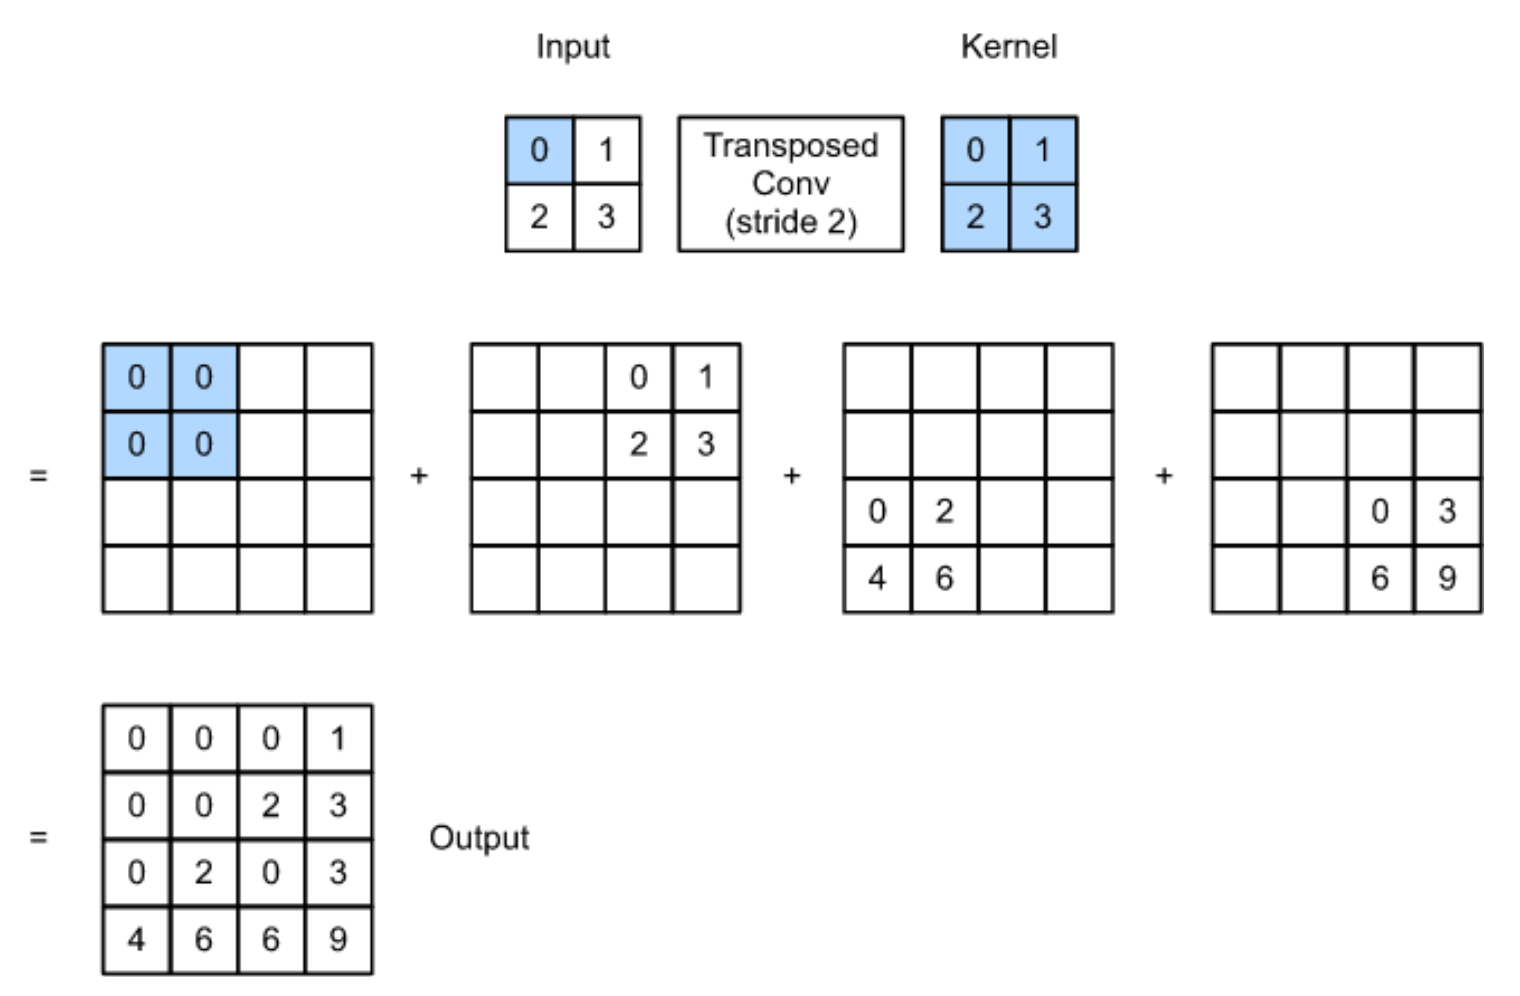
\includegraphics[scale=0.2]{Transposed Convolution With stride .png}
    \caption{Transposed Convolution with Stride}
    \label{}
\end{figure}\end{center}
For a image $n\times n$ with filter $f\times f$, padding $p$ and stride $s$, the dimension of the output is
\begin{equation}
    \begin{aligned}
        (s(n-1)+f-2p)\times (s(n-1)+f-2p)
    \end{aligned}
    \nonumber
\end{equation}
















































\end{document}